\chapter{Evaluation} \label{chap:evaluation}

\section{Data} \label{sec:data}

The data consists of many sequences of unsigned integers known as \textit{reads}. Each integer represents the quantised ionic current recorded at a certain time step as a single-stranded DNA or RNA molecule is driven through a nanoscale protein pore (or \textit{nanopore}) \cite{Wang2021}. Disturbances in the ionic current caused by the molecule's biological structure can be used to determine its nucleic acid sequence.

Let each read be represented by
\[ x := (x_i\mid x_i \in \mathbb{Z} \cap [0, 2^{16})) \]
where $i\in \mathbb{Z}\cap [0, n)$. Computationally, $x$ is an unsigned 16-bit integer array with $n$ elements. However, in practice the full range of $2^{16}$ integers is never met.

For the remainder of the thesis, the data which we will use for analysing the characteristics of nanopore signal data and for comparing compression methods is the NA12878 data set. The data set has been well studied and is used prolifically for benchmarking genomics tools. The data set originates from a Utah woman. Her DNA sample was artificially recreated, treated using a short read eliminator kit and sequenced on an ONT PromethION 48. This device produces the most data out of all nanopore sequencing devices so is most appropriate for data compression.
%TODO actually 48?

The data set consists of \num{500000} reads and $\sim$ 57 billion signal points. Altogether the data set is $\sim$39 GiB when stored in the BLOW5 file format (v0.2.0) using svb-zd (differential followed by zig-zag encoding and Stream VByte) signal compression and zlib record compression. See Table \ref{tab:data} for an overview of the data set.

\begin{table}
    \caption{\label{tab:data}The NA12878 data set.}
    \begin{tabular}{|l|l|}
        \hline
        Description & Adult Utah Female DNA\\
        \hline
	Sequencer & ONT PromethION\\
	Start time (ISO 8601) & 2020-10-27T05:41:50Z\\
	No. of reads & \num{500000}\\
	No. of signals ($\times 10^9$) & $\sim$ 57\\
	Avg. read length & $\sim$ \num{113471}\\
        \hline
	Gibibytes (in BLOW5 v0.2.0) & $\sim$ 39\\
	\hline
    \end{tabular}
\end{table}


The raw signal values in the data set range from 158 to 1748 with a median of 474 and standard deviation of $\sim$ 35. The maximum is 1748 but the middle 99\% of the data ranges from 350 to 622. Figure \ref{fig:data-hist} shows the singular-width bin histogram of the raw signal values between 295 and 687.
As one can observe, the distribution is fairly symmetric around the centre with the median and mean very close to one another. However, it is slightly right-skewed with its right tail extending much further than its left. This is most evident by observing that the maximum is more than four times further from the median than the minimum.
Most interestingly, there is clearly a cyclical pattern in the relative frequency of adjacent signal points which repeats every 16 values.
%TODO put closeup figure showing pattern
This is most likely due to the nature of the analogue-to-digital converter (ADC) which digitises the analogue ionic current signal during sequencing.

\begin{table}
    \caption{\label{tab:rawsig} Summary statistics of the data's raw signal values.}
    \begin{tabular}{|l|l|}
        \hline
Min & 158\\
	    Q1 & 439\\

Q2 & 474\\
	    Q3 & 511\\
Max & 1748\\
\hline
Mean & 475.2245\\
	    Mode & 487\\
SD & 35.0675\\
	\hline
    \end{tabular}
\end{table}

\begin{figure}
	\centering
% Created by tikzDevice version 0.12.3.1 on 2022-09-19 10:24:26
% !TEX encoding = UTF-8 Unicode
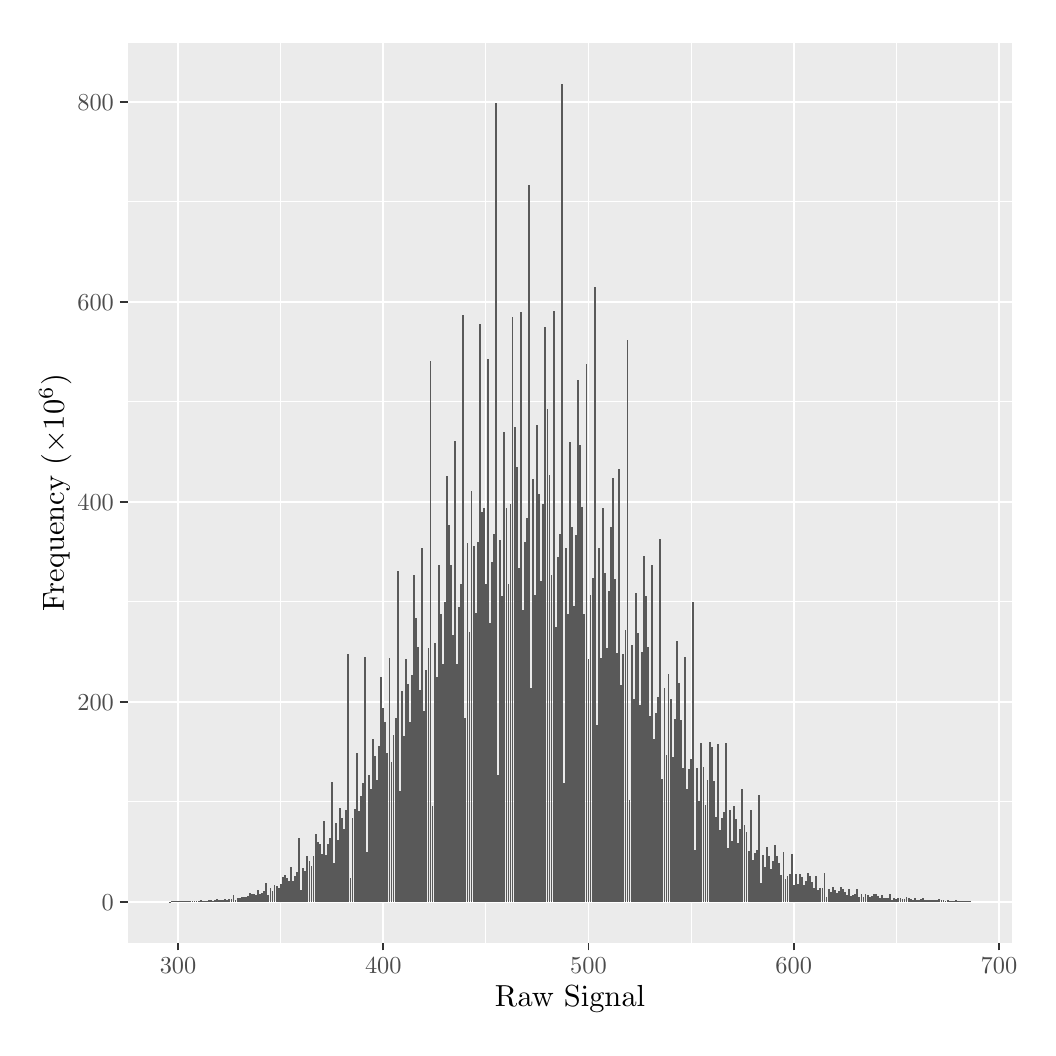
\begin{tikzpicture}[x=1pt,y=1pt]
\definecolor{fillColor}{RGB}{255,255,255}
\path[use as bounding box,fill=fillColor,fill opacity=0.00] (0,0) rectangle (361.35,361.35);
\begin{scope}
\path[clip] (  0.00,  0.00) rectangle (361.35,361.35);
\definecolor{drawColor}{RGB}{255,255,255}
\definecolor{fillColor}{RGB}{255,255,255}

\path[draw=drawColor,line width= 0.6pt,line join=round,line cap=round,fill=fillColor] (  0.00,  0.00) rectangle (361.35,361.35);
\end{scope}
\begin{scope}
\path[clip] ( 36.11, 30.69) rectangle (355.85,355.85);
\definecolor{fillColor}{gray}{0.92}

\path[fill=fillColor] ( 36.11, 30.69) rectangle (355.85,355.85);
\definecolor{drawColor}{RGB}{255,255,255}

\path[draw=drawColor,line width= 0.3pt,line join=round] ( 36.11, 81.60) --
	(355.85, 81.60);

\path[draw=drawColor,line width= 0.3pt,line join=round] ( 36.11,153.87) --
	(355.85,153.87);

\path[draw=drawColor,line width= 0.3pt,line join=round] ( 36.11,226.14) --
	(355.85,226.14);

\path[draw=drawColor,line width= 0.3pt,line join=round] ( 36.11,298.41) --
	(355.85,298.41);

\path[draw=drawColor,line width= 0.3pt,line join=round] ( 91.43, 30.69) --
	( 91.43,355.85);

\path[draw=drawColor,line width= 0.3pt,line join=round] (165.58, 30.69) --
	(165.58,355.85);

\path[draw=drawColor,line width= 0.3pt,line join=round] (239.73, 30.69) --
	(239.73,355.85);

\path[draw=drawColor,line width= 0.3pt,line join=round] (313.88, 30.69) --
	(313.88,355.85);

\path[draw=drawColor,line width= 0.6pt,line join=round] ( 36.11, 45.47) --
	(355.85, 45.47);

\path[draw=drawColor,line width= 0.6pt,line join=round] ( 36.11,117.73) --
	(355.85,117.73);

\path[draw=drawColor,line width= 0.6pt,line join=round] ( 36.11,190.00) --
	(355.85,190.00);

\path[draw=drawColor,line width= 0.6pt,line join=round] ( 36.11,262.27) --
	(355.85,262.27);

\path[draw=drawColor,line width= 0.6pt,line join=round] ( 36.11,334.54) --
	(355.85,334.54);

\path[draw=drawColor,line width= 0.6pt,line join=round] ( 54.35, 30.69) --
	( 54.35,355.85);

\path[draw=drawColor,line width= 0.6pt,line join=round] (128.50, 30.69) --
	(128.50,355.85);

\path[draw=drawColor,line width= 0.6pt,line join=round] (202.65, 30.69) --
	(202.65,355.85);

\path[draw=drawColor,line width= 0.6pt,line join=round] (276.81, 30.69) --
	(276.81,355.85);

\path[draw=drawColor,line width= 0.6pt,line join=round] (350.96, 30.69) --
	(350.96,355.85);
\definecolor{fillColor}{gray}{0.35}

\path[fill=fillColor] ( 51.05, 45.47) rectangle ( 51.72, 45.53);

\path[fill=fillColor] ( 51.79, 45.47) rectangle ( 52.46, 45.66);

\path[fill=fillColor] ( 52.54, 45.47) rectangle ( 53.20, 45.64);

\path[fill=fillColor] ( 53.28, 45.47) rectangle ( 53.94, 45.72);

\path[fill=fillColor] ( 54.02, 45.47) rectangle ( 54.69, 45.69);

\path[fill=fillColor] ( 54.76, 45.47) rectangle ( 55.43, 45.65);

\path[fill=fillColor] ( 55.50, 45.47) rectangle ( 56.17, 45.71);

\path[fill=fillColor] ( 56.24, 45.47) rectangle ( 56.91, 45.80);

\path[fill=fillColor] ( 56.98, 45.47) rectangle ( 57.65, 45.79);

\path[fill=fillColor] ( 57.73, 45.47) rectangle ( 58.39, 45.75);

\path[fill=fillColor] ( 58.47, 45.47) rectangle ( 59.14, 45.71);

\path[fill=fillColor] ( 59.21, 45.47) rectangle ( 59.88, 45.88);

\path[fill=fillColor] ( 59.95, 45.47) rectangle ( 60.62, 45.70);

\path[fill=fillColor] ( 60.69, 45.47) rectangle ( 61.36, 45.76);

\path[fill=fillColor] ( 61.43, 45.47) rectangle ( 62.10, 45.80);

\path[fill=fillColor] ( 62.18, 45.47) rectangle ( 62.84, 46.10);

\path[fill=fillColor] ( 62.92, 45.47) rectangle ( 63.58, 45.69);

\path[fill=fillColor] ( 63.66, 45.47) rectangle ( 64.33, 45.90);

\path[fill=fillColor] ( 64.40, 45.47) rectangle ( 65.07, 45.83);

\path[fill=fillColor] ( 65.14, 45.47) rectangle ( 65.81, 46.01);

\path[fill=fillColor] ( 65.88, 45.47) rectangle ( 66.55, 45.99);

\path[fill=fillColor] ( 66.62, 45.47) rectangle ( 67.29, 45.92);

\path[fill=fillColor] ( 67.37, 45.47) rectangle ( 68.03, 46.06);

\path[fill=fillColor] ( 68.11, 45.47) rectangle ( 68.77, 46.40);

\path[fill=fillColor] ( 68.85, 45.47) rectangle ( 69.52, 46.28);

\path[fill=fillColor] ( 69.59, 45.47) rectangle ( 70.26, 46.26);

\path[fill=fillColor] ( 70.33, 45.47) rectangle ( 71.00, 46.19);

\path[fill=fillColor] ( 71.07, 45.47) rectangle ( 71.74, 46.62);

\path[fill=fillColor] ( 71.81, 45.47) rectangle ( 72.48, 46.25);

\path[fill=fillColor] ( 72.56, 45.47) rectangle ( 73.22, 46.38);

\path[fill=fillColor] ( 73.30, 45.47) rectangle ( 73.97, 46.55);

\path[fill=fillColor] ( 74.04, 45.47) rectangle ( 74.71, 47.78);

\path[fill=fillColor] ( 74.78, 45.47) rectangle ( 75.45, 45.99);

\path[fill=fillColor] ( 75.52, 45.47) rectangle ( 76.19, 46.82);

\path[fill=fillColor] ( 76.26, 45.47) rectangle ( 76.93, 46.72);

\path[fill=fillColor] ( 77.01, 45.47) rectangle ( 77.67, 47.31);

\path[fill=fillColor] ( 77.75, 45.47) rectangle ( 78.41, 47.27);

\path[fill=fillColor] ( 78.49, 45.47) rectangle ( 79.16, 47.05);

\path[fill=fillColor] ( 79.23, 45.47) rectangle ( 79.90, 47.59);

\path[fill=fillColor] ( 79.97, 45.47) rectangle ( 80.64, 48.70);

\path[fill=fillColor] ( 80.71, 45.47) rectangle ( 81.38, 48.39);

\path[fill=fillColor] ( 81.45, 45.47) rectangle ( 82.12, 48.37);

\path[fill=fillColor] ( 82.20, 45.47) rectangle ( 82.86, 48.01);

\path[fill=fillColor] ( 82.94, 45.47) rectangle ( 83.60, 49.59);

\path[fill=fillColor] ( 83.68, 45.47) rectangle ( 84.35, 48.22);

\path[fill=fillColor] ( 84.42, 45.47) rectangle ( 85.09, 48.75);

\path[fill=fillColor] ( 85.16, 45.47) rectangle ( 85.83, 49.25);

\path[fill=fillColor] ( 85.90, 45.47) rectangle ( 86.57, 52.42);

\path[fill=fillColor] ( 86.65, 45.47) rectangle ( 87.31, 48.00);

\path[fill=fillColor] ( 87.39, 45.47) rectangle ( 88.05, 50.43);

\path[fill=fillColor] ( 88.13, 45.47) rectangle ( 88.80, 49.56);

\path[fill=fillColor] ( 88.87, 45.47) rectangle ( 89.54, 51.51);

\path[fill=fillColor] ( 89.61, 45.47) rectangle ( 90.28, 51.28);

\path[fill=fillColor] ( 90.35, 45.47) rectangle ( 91.02, 50.52);

\path[fill=fillColor] ( 91.09, 45.47) rectangle ( 91.76, 52.07);

\path[fill=fillColor] ( 91.84, 45.47) rectangle ( 92.50, 54.53);

\path[fill=fillColor] ( 92.58, 45.47) rectangle ( 93.24, 55.33);

\path[fill=fillColor] ( 93.32, 45.47) rectangle ( 93.99, 54.12);

\path[fill=fillColor] ( 94.06, 45.47) rectangle ( 94.73, 53.02);

\path[fill=fillColor] ( 94.80, 45.47) rectangle ( 95.47, 57.88);

\path[fill=fillColor] ( 95.54, 45.47) rectangle ( 96.21, 53.16);

\path[fill=fillColor] ( 96.28, 45.47) rectangle ( 96.95, 54.86);

\path[fill=fillColor] ( 97.03, 45.47) rectangle ( 97.69, 56.14);

\path[fill=fillColor] ( 97.77, 45.47) rectangle ( 98.44, 68.59);

\path[fill=fillColor] ( 98.51, 45.47) rectangle ( 99.18, 49.85);

\path[fill=fillColor] ( 99.25, 45.47) rectangle ( 99.92, 57.84);

\path[fill=fillColor] ( 99.99, 45.47) rectangle (100.66, 56.51);

\path[fill=fillColor] (100.73, 45.47) rectangle (101.40, 61.93);

\path[fill=fillColor] (101.48, 45.47) rectangle (102.14, 60.27);

\path[fill=fillColor] (102.22, 45.47) rectangle (102.88, 58.38);

\path[fill=fillColor] (102.96, 45.47) rectangle (103.63, 62.08);

\path[fill=fillColor] (103.70, 45.47) rectangle (104.37, 70.01);

\path[fill=fillColor] (104.44, 45.47) rectangle (105.11, 67.13);

\path[fill=fillColor] (105.18, 45.47) rectangle (105.85, 66.29);

\path[fill=fillColor] (105.92, 45.47) rectangle (106.59, 62.77);

\path[fill=fillColor] (106.67, 45.47) rectangle (107.33, 74.50);

\path[fill=fillColor] (107.41, 45.47) rectangle (108.07, 62.37);

\path[fill=fillColor] (108.15, 45.47) rectangle (108.82, 66.45);

\path[fill=fillColor] (108.89, 45.47) rectangle (109.56, 68.66);

\path[fill=fillColor] (109.63, 45.47) rectangle (110.30, 88.95);

\path[fill=fillColor] (110.37, 45.47) rectangle (111.04, 59.40);

\path[fill=fillColor] (111.11, 45.47) rectangle (111.78, 74.03);

\path[fill=fillColor] (111.86, 45.47) rectangle (112.52, 67.97);

\path[fill=fillColor] (112.60, 45.47) rectangle (113.27, 79.49);

\path[fill=fillColor] (113.34, 45.47) rectangle (114.01, 75.93);

\path[fill=fillColor] (114.08, 45.47) rectangle (114.75, 71.63);

\path[fill=fillColor] (114.82, 45.47) rectangle (115.49, 78.62);

\path[fill=fillColor] (115.56, 45.47) rectangle (116.23,135.08);

\path[fill=fillColor] (116.31, 45.47) rectangle (116.97, 54.11);

\path[fill=fillColor] (117.05, 45.47) rectangle (117.71, 75.70);

\path[fill=fillColor] (117.79, 45.47) rectangle (118.46, 79.05);

\path[fill=fillColor] (118.53, 45.47) rectangle (119.20, 99.15);

\path[fill=fillColor] (119.27, 45.47) rectangle (119.94, 78.20);

\path[fill=fillColor] (120.01, 45.47) rectangle (120.68, 83.67);

\path[fill=fillColor] (120.75, 45.47) rectangle (121.42, 88.49);

\path[fill=fillColor] (121.50, 45.47) rectangle (122.16,133.84);

\path[fill=fillColor] (122.24, 45.47) rectangle (122.90, 63.33);

\path[fill=fillColor] (122.98, 45.47) rectangle (123.65, 91.15);

\path[fill=fillColor] (123.72, 45.47) rectangle (124.39, 86.16);

\path[fill=fillColor] (124.46, 45.47) rectangle (125.13,104.13);

\path[fill=fillColor] (125.20, 45.47) rectangle (125.87, 98.07);

\path[fill=fillColor] (125.95, 45.47) rectangle (126.61, 89.47);

\path[fill=fillColor] (126.69, 45.47) rectangle (127.35,101.74);

\path[fill=fillColor] (127.43, 45.47) rectangle (128.10,126.65);

\path[fill=fillColor] (128.17, 45.47) rectangle (128.84,115.37);

\path[fill=fillColor] (128.91, 45.47) rectangle (129.58,110.28);

\path[fill=fillColor] (129.65, 45.47) rectangle (130.32, 99.28);

\path[fill=fillColor] (130.39, 45.47) rectangle (131.06,133.47);

\path[fill=fillColor] (131.14, 45.47) rectangle (131.80, 96.00);

\path[fill=fillColor] (131.88, 45.47) rectangle (132.54,105.80);

\path[fill=fillColor] (132.62, 45.47) rectangle (133.29,111.94);

\path[fill=fillColor] (133.36, 45.47) rectangle (134.03,164.97);

\path[fill=fillColor] (134.10, 45.47) rectangle (134.77, 85.65);

\path[fill=fillColor] (134.84, 45.47) rectangle (135.51,121.61);

\path[fill=fillColor] (135.58, 45.47) rectangle (136.25,105.35);

\path[fill=fillColor] (136.33, 45.47) rectangle (136.99,133.30);

\path[fill=fillColor] (137.07, 45.47) rectangle (137.74,124.36);

\path[fill=fillColor] (137.81, 45.47) rectangle (138.48,110.32);

\path[fill=fillColor] (138.55, 45.47) rectangle (139.22,127.37);

\path[fill=fillColor] (139.29, 45.47) rectangle (139.96,163.46);

\path[fill=fillColor] (140.03, 45.47) rectangle (140.70,148.19);

\path[fill=fillColor] (140.78, 45.47) rectangle (141.44,137.58);

\path[fill=fillColor] (141.52, 45.47) rectangle (142.18,122.15);

\path[fill=fillColor] (142.26, 45.47) rectangle (142.93,173.21);

\path[fill=fillColor] (143.00, 45.47) rectangle (143.67,114.39);

\path[fill=fillColor] (143.74, 45.47) rectangle (144.41,129.26);

\path[fill=fillColor] (144.48, 45.47) rectangle (145.15,137.31);

\path[fill=fillColor] (145.22, 45.47) rectangle (145.89,240.76);

\path[fill=fillColor] (145.97, 45.47) rectangle (146.63, 80.01);

\path[fill=fillColor] (146.71, 45.47) rectangle (147.37,139.16);

\path[fill=fillColor] (147.45, 45.47) rectangle (148.12,126.64);

\path[fill=fillColor] (148.19, 45.47) rectangle (148.86,167.15);

\path[fill=fillColor] (148.93, 45.47) rectangle (149.60,149.44);

\path[fill=fillColor] (149.67, 45.47) rectangle (150.34,131.32);

\path[fill=fillColor] (150.41, 45.47) rectangle (151.08,153.71);

\path[fill=fillColor] (151.16, 45.47) rectangle (151.82,199.18);

\path[fill=fillColor] (151.90, 45.47) rectangle (152.57,181.51);

\path[fill=fillColor] (152.64, 45.47) rectangle (153.31,167.09);

\path[fill=fillColor] (153.38, 45.47) rectangle (154.05,142.01);

\path[fill=fillColor] (154.12, 45.47) rectangle (154.79,211.90);

\path[fill=fillColor] (154.86, 45.47) rectangle (155.53,131.59);

\path[fill=fillColor] (155.61, 45.47) rectangle (156.27,151.91);

\path[fill=fillColor] (156.35, 45.47) rectangle (157.01,160.29);

\path[fill=fillColor] (157.09, 45.47) rectangle (157.76,257.39);

\path[fill=fillColor] (157.83, 45.47) rectangle (158.50,111.83);

\path[fill=fillColor] (158.57, 45.47) rectangle (159.24,175.08);

\path[fill=fillColor] (159.31, 45.47) rectangle (159.98,143.03);

\path[fill=fillColor] (160.05, 45.47) rectangle (160.72,194.08);

\path[fill=fillColor] (160.80, 45.47) rectangle (161.46,174.21);

\path[fill=fillColor] (161.54, 45.47) rectangle (162.20,149.77);

\path[fill=fillColor] (162.28, 45.47) rectangle (162.95,175.60);

\path[fill=fillColor] (163.02, 45.47) rectangle (163.69,254.37);

\path[fill=fillColor] (163.76, 45.47) rectangle (164.43,186.26);

\path[fill=fillColor] (164.50, 45.47) rectangle (165.17,187.93);

\path[fill=fillColor] (165.25, 45.47) rectangle (165.91,160.33);

\path[fill=fillColor] (165.99, 45.47) rectangle (166.65,241.64);

\path[fill=fillColor] (166.73, 45.47) rectangle (167.40,146.40);

\path[fill=fillColor] (167.47, 45.47) rectangle (168.14,168.14);

\path[fill=fillColor] (168.21, 45.47) rectangle (168.88,178.30);

\path[fill=fillColor] (168.95, 45.47) rectangle (169.62,334.23);

\path[fill=fillColor] (169.69, 45.47) rectangle (170.36, 91.26);

\path[fill=fillColor] (170.44, 45.47) rectangle (171.10,176.09);

\path[fill=fillColor] (171.18, 45.47) rectangle (171.84,156.13);

\path[fill=fillColor] (171.92, 45.47) rectangle (172.59,215.23);

\path[fill=fillColor] (172.66, 45.47) rectangle (173.33,187.91);

\path[fill=fillColor] (173.40, 45.47) rectangle (174.07,160.40);

\path[fill=fillColor] (174.14, 45.47) rectangle (174.81,189.26);

\path[fill=fillColor] (174.88, 45.47) rectangle (175.55,256.67);

\path[fill=fillColor] (175.63, 45.47) rectangle (176.29,216.88);

\path[fill=fillColor] (176.37, 45.47) rectangle (177.04,202.71);

\path[fill=fillColor] (177.11, 45.47) rectangle (177.78,166.03);

\path[fill=fillColor] (177.85, 45.47) rectangle (178.52,258.56);

\path[fill=fillColor] (178.59, 45.47) rectangle (179.26,151.03);

\path[fill=fillColor] (179.33, 45.47) rectangle (180.00,175.36);

\path[fill=fillColor] (180.08, 45.47) rectangle (180.74,184.25);

\path[fill=fillColor] (180.82, 45.47) rectangle (181.48,304.67);

\path[fill=fillColor] (181.56, 45.47) rectangle (182.23,122.72);

\path[fill=fillColor] (182.30, 45.47) rectangle (182.97,198.20);

\path[fill=fillColor] (183.04, 45.47) rectangle (183.71,156.32);

\path[fill=fillColor] (183.78, 45.47) rectangle (184.45,217.62);

\path[fill=fillColor] (184.52, 45.47) rectangle (185.19,193.02);

\path[fill=fillColor] (185.27, 45.47) rectangle (185.93,161.40);

\path[fill=fillColor] (186.01, 45.47) rectangle (186.67,189.34);

\path[fill=fillColor] (186.75, 45.47) rectangle (187.42,253.05);

\path[fill=fillColor] (187.49, 45.47) rectangle (188.16,223.56);

\path[fill=fillColor] (188.23, 45.47) rectangle (188.90,199.76);

\path[fill=fillColor] (188.97, 45.47) rectangle (189.64,163.73);

\path[fill=fillColor] (189.71, 45.47) rectangle (190.38,258.86);

\path[fill=fillColor] (190.46, 45.47) rectangle (191.12,144.96);

\path[fill=fillColor] (191.20, 45.47) rectangle (191.87,170.12);

\path[fill=fillColor] (191.94, 45.47) rectangle (192.61,178.35);

\path[fill=fillColor] (192.68, 45.47) rectangle (193.35,341.07);

\path[fill=fillColor] (193.42, 45.47) rectangle (194.09, 88.36);

\path[fill=fillColor] (194.16, 45.47) rectangle (194.83,173.31);

\path[fill=fillColor] (194.91, 45.47) rectangle (195.57,149.64);

\path[fill=fillColor] (195.65, 45.47) rectangle (196.31,211.61);

\path[fill=fillColor] (196.39, 45.47) rectangle (197.06,180.78);

\path[fill=fillColor] (197.13, 45.47) rectangle (197.80,152.35);

\path[fill=fillColor] (197.87, 45.47) rectangle (198.54,178.14);

\path[fill=fillColor] (198.61, 45.47) rectangle (199.28,234.09);

\path[fill=fillColor] (199.35, 45.47) rectangle (200.02,210.38);

\path[fill=fillColor] (200.10, 45.47) rectangle (200.76,188.10);

\path[fill=fillColor] (200.84, 45.47) rectangle (201.50,149.59);

\path[fill=fillColor] (201.58, 45.47) rectangle (202.25,239.72);

\path[fill=fillColor] (202.32, 45.47) rectangle (202.99,133.34);

\path[fill=fillColor] (203.06, 45.47) rectangle (203.73,156.48);

\path[fill=fillColor] (203.80, 45.47) rectangle (204.47,162.53);

\path[fill=fillColor] (204.55, 45.47) rectangle (205.21,267.80);

\path[fill=fillColor] (205.29, 45.47) rectangle (205.95,109.31);

\path[fill=fillColor] (206.03, 45.47) rectangle (206.70,173.18);

\path[fill=fillColor] (206.77, 45.47) rectangle (207.44,133.53);

\path[fill=fillColor] (207.51, 45.47) rectangle (208.18,187.81);

\path[fill=fillColor] (208.25, 45.47) rectangle (208.92,164.45);

\path[fill=fillColor] (208.99, 45.47) rectangle (209.66,137.06);

\path[fill=fillColor] (209.74, 45.47) rectangle (210.40,157.80);

\path[fill=fillColor] (210.48, 45.47) rectangle (211.14,180.99);

\path[fill=fillColor] (211.22, 45.47) rectangle (211.89,198.58);

\path[fill=fillColor] (211.96, 45.47) rectangle (212.63,162.15);

\path[fill=fillColor] (212.70, 45.47) rectangle (213.37,135.28);

\path[fill=fillColor] (213.44, 45.47) rectangle (214.11,201.77);

\path[fill=fillColor] (214.18, 45.47) rectangle (214.85,123.84);

\path[fill=fillColor] (214.93, 45.47) rectangle (215.59,135.12);

\path[fill=fillColor] (215.67, 45.47) rectangle (216.34,143.70);

\path[fill=fillColor] (216.41, 45.47) rectangle (217.08,248.59);

\path[fill=fillColor] (217.15, 45.47) rectangle (217.82, 82.28);

\path[fill=fillColor] (217.89, 45.47) rectangle (218.56,138.27);

\path[fill=fillColor] (218.63, 45.47) rectangle (219.30,118.76);

\path[fill=fillColor] (219.38, 45.47) rectangle (220.04,157.22);

\path[fill=fillColor] (220.12, 45.47) rectangle (220.78,142.78);

\path[fill=fillColor] (220.86, 45.47) rectangle (221.53,116.77);

\path[fill=fillColor] (221.60, 45.47) rectangle (222.27,135.82);

\path[fill=fillColor] (222.34, 45.47) rectangle (223.01,170.53);

\path[fill=fillColor] (223.08, 45.47) rectangle (223.75,155.96);

\path[fill=fillColor] (223.82, 45.47) rectangle (224.49,137.45);

\path[fill=fillColor] (224.57, 45.47) rectangle (225.23,112.77);

\path[fill=fillColor] (225.31, 45.47) rectangle (225.97,167.15);

\path[fill=fillColor] (226.05, 45.47) rectangle (226.72,104.37);

\path[fill=fillColor] (226.79, 45.47) rectangle (227.46,113.79);

\path[fill=fillColor] (227.53, 45.47) rectangle (228.20,119.46);

\path[fill=fillColor] (228.27, 45.47) rectangle (228.94,176.54);

\path[fill=fillColor] (229.01, 45.47) rectangle (229.68, 89.95);

\path[fill=fillColor] (229.76, 45.47) rectangle (230.42,122.88);

\path[fill=fillColor] (230.50, 45.47) rectangle (231.17, 98.54);

\path[fill=fillColor] (231.24, 45.47) rectangle (231.91,127.73);

\path[fill=fillColor] (231.98, 45.47) rectangle (232.65,118.61);

\path[fill=fillColor] (232.72, 45.47) rectangle (233.39, 97.89);

\path[fill=fillColor] (233.46, 45.47) rectangle (234.13,111.36);

\path[fill=fillColor] (234.21, 45.47) rectangle (234.87,139.57);

\path[fill=fillColor] (234.95, 45.47) rectangle (235.61,124.40);

\path[fill=fillColor] (235.69, 45.47) rectangle (236.36,111.29);

\path[fill=fillColor] (236.43, 45.47) rectangle (237.10, 93.71);

\path[fill=fillColor] (237.17, 45.47) rectangle (237.84,133.82);

\path[fill=fillColor] (237.91, 45.47) rectangle (238.58, 86.25);

\path[fill=fillColor] (238.65, 45.47) rectangle (239.32, 93.32);

\path[fill=fillColor] (239.40, 45.47) rectangle (240.06, 97.23);

\path[fill=fillColor] (240.14, 45.47) rectangle (240.80,153.65);

\path[fill=fillColor] (240.88, 45.47) rectangle (241.55, 64.06);

\path[fill=fillColor] (241.62, 45.47) rectangle (242.29, 93.74);

\path[fill=fillColor] (242.36, 45.47) rectangle (243.03, 81.86);

\path[fill=fillColor] (243.10, 45.47) rectangle (243.77,102.75);

\path[fill=fillColor] (243.85, 45.47) rectangle (244.51, 94.05);

\path[fill=fillColor] (244.59, 45.47) rectangle (245.25, 80.49);

\path[fill=fillColor] (245.33, 45.47) rectangle (246.00, 89.36);

\path[fill=fillColor] (246.07, 45.47) rectangle (246.74,103.28);

\path[fill=fillColor] (246.81, 45.47) rectangle (247.48,101.45);

\path[fill=fillColor] (247.55, 45.47) rectangle (248.22, 89.00);

\path[fill=fillColor] (248.29, 45.47) rectangle (248.96, 75.95);

\path[fill=fillColor] (249.04, 45.47) rectangle (249.70,102.58);

\path[fill=fillColor] (249.78, 45.47) rectangle (250.44, 71.25);

\path[fill=fillColor] (250.52, 45.47) rectangle (251.19, 75.86);

\path[fill=fillColor] (251.26, 45.47) rectangle (251.93, 77.94);

\path[fill=fillColor] (252.00, 45.47) rectangle (252.67,102.76);

\path[fill=fillColor] (252.74, 45.47) rectangle (253.41, 64.79);

\path[fill=fillColor] (253.48, 45.47) rectangle (254.15, 78.69);

\path[fill=fillColor] (254.23, 45.47) rectangle (254.89, 67.34);

\path[fill=fillColor] (254.97, 45.47) rectangle (255.64, 80.10);

\path[fill=fillColor] (255.71, 45.47) rectangle (256.38, 75.49);

\path[fill=fillColor] (256.45, 45.47) rectangle (257.12, 66.71);

\path[fill=fillColor] (257.19, 45.47) rectangle (257.86, 71.82);

\path[fill=fillColor] (257.93, 45.47) rectangle (258.60, 86.17);

\path[fill=fillColor] (258.68, 45.47) rectangle (259.34, 73.06);

\path[fill=fillColor] (259.42, 45.47) rectangle (260.08, 70.86);

\path[fill=fillColor] (260.16, 45.47) rectangle (260.83, 63.66);

\path[fill=fillColor] (260.90, 45.47) rectangle (261.57, 78.67);

\path[fill=fillColor] (261.64, 45.47) rectangle (262.31, 60.75);

\path[fill=fillColor] (262.38, 45.47) rectangle (263.05, 63.01);

\path[fill=fillColor] (263.12, 45.47) rectangle (263.79, 64.32);

\path[fill=fillColor] (263.87, 45.47) rectangle (264.53, 84.13);

\path[fill=fillColor] (264.61, 45.47) rectangle (265.27, 52.13);

\path[fill=fillColor] (265.35, 45.47) rectangle (266.02, 62.54);

\path[fill=fillColor] (266.09, 45.47) rectangle (266.76, 58.03);

\path[fill=fillColor] (266.83, 45.47) rectangle (267.50, 65.13);

\path[fill=fillColor] (267.57, 45.47) rectangle (268.24, 62.08);

\path[fill=fillColor] (268.31, 45.47) rectangle (268.98, 57.30);

\path[fill=fillColor] (269.06, 45.47) rectangle (269.72, 60.10);

\path[fill=fillColor] (269.80, 45.47) rectangle (270.47, 66.11);

\path[fill=fillColor] (270.54, 45.47) rectangle (271.21, 62.16);

\path[fill=fillColor] (271.28, 45.47) rectangle (271.95, 59.49);

\path[fill=fillColor] (272.02, 45.47) rectangle (272.69, 55.17);

\path[fill=fillColor] (272.76, 45.47) rectangle (273.43, 63.34);

\path[fill=fillColor] (273.51, 45.47) rectangle (274.17, 53.68);

\path[fill=fillColor] (274.25, 45.47) rectangle (274.91, 54.91);

\path[fill=fillColor] (274.99, 45.47) rectangle (275.66, 55.50);

\path[fill=fillColor] (275.73, 45.47) rectangle (276.40, 62.73);

\path[fill=fillColor] (276.47, 45.47) rectangle (277.14, 51.45);

\path[fill=fillColor] (277.21, 45.47) rectangle (277.88, 55.45);

\path[fill=fillColor] (277.95, 45.47) rectangle (278.62, 52.00);

\path[fill=fillColor] (278.70, 45.47) rectangle (279.36, 55.64);

\path[fill=fillColor] (279.44, 45.47) rectangle (280.10, 54.29);

\path[fill=fillColor] (280.18, 45.47) rectangle (280.85, 51.70);

\path[fill=fillColor] (280.92, 45.47) rectangle (281.59, 53.08);

\path[fill=fillColor] (281.66, 45.47) rectangle (282.33, 55.79);

\path[fill=fillColor] (282.40, 45.47) rectangle (283.07, 54.67);

\path[fill=fillColor] (283.15, 45.47) rectangle (283.81, 52.66);

\path[fill=fillColor] (283.89, 45.47) rectangle (284.55, 50.55);

\path[fill=fillColor] (284.63, 45.47) rectangle (285.30, 54.72);

\path[fill=fillColor] (285.37, 45.47) rectangle (286.04, 49.67);

\path[fill=fillColor] (286.11, 45.47) rectangle (286.78, 50.33);

\path[fill=fillColor] (286.85, 45.47) rectangle (287.52, 50.64);

\path[fill=fillColor] (287.59, 45.47) rectangle (288.26, 55.81);

\path[fill=fillColor] (288.34, 45.47) rectangle (289.00, 47.38);

\path[fill=fillColor] (289.08, 45.47) rectangle (289.74, 50.16);

\path[fill=fillColor] (289.82, 45.47) rectangle (290.49, 48.88);

\path[fill=fillColor] (290.56, 45.47) rectangle (291.23, 50.77);

\path[fill=fillColor] (291.30, 45.47) rectangle (291.97, 49.90);

\path[fill=fillColor] (292.04, 45.47) rectangle (292.71, 48.68);

\path[fill=fillColor] (292.78, 45.47) rectangle (293.45, 49.38);

\path[fill=fillColor] (293.53, 45.47) rectangle (294.19, 50.66);

\path[fill=fillColor] (294.27, 45.47) rectangle (294.94, 50.20);

\path[fill=fillColor] (295.01, 45.47) rectangle (295.68, 49.20);

\path[fill=fillColor] (295.75, 45.47) rectangle (296.42, 48.06);

\path[fill=fillColor] (296.49, 45.47) rectangle (297.16, 50.20);

\path[fill=fillColor] (297.23, 45.47) rectangle (297.90, 47.66);

\path[fill=fillColor] (297.98, 45.47) rectangle (298.64, 48.00);

\path[fill=fillColor] (298.72, 45.47) rectangle (299.38, 48.15);

\path[fill=fillColor] (299.46, 45.47) rectangle (300.13, 50.00);

\path[fill=fillColor] (300.20, 45.47) rectangle (300.87, 47.12);

\path[fill=fillColor] (300.94, 45.47) rectangle (301.61, 48.16);

\path[fill=fillColor] (301.68, 45.47) rectangle (302.35, 47.24);

\path[fill=fillColor] (302.42, 45.47) rectangle (303.09, 48.21);

\path[fill=fillColor] (303.17, 45.47) rectangle (303.83, 47.84);

\path[fill=fillColor] (303.91, 45.47) rectangle (304.57, 47.19);

\path[fill=fillColor] (304.65, 45.47) rectangle (305.32, 47.54);

\path[fill=fillColor] (305.39, 45.47) rectangle (306.06, 48.13);

\path[fill=fillColor] (306.13, 45.47) rectangle (306.80, 48.23);

\path[fill=fillColor] (306.87, 45.47) rectangle (307.54, 47.44);

\path[fill=fillColor] (307.61, 45.47) rectangle (308.28, 46.91);

\path[fill=fillColor] (308.36, 45.47) rectangle (309.02, 47.94);

\path[fill=fillColor] (309.10, 45.47) rectangle (309.77, 46.74);

\path[fill=fillColor] (309.84, 45.47) rectangle (310.51, 46.85);

\path[fill=fillColor] (310.58, 45.47) rectangle (311.25, 46.96);

\path[fill=fillColor] (311.32, 45.47) rectangle (311.99, 48.27);

\path[fill=fillColor] (312.06, 45.47) rectangle (312.73, 46.12);

\path[fill=fillColor] (312.81, 45.47) rectangle (313.47, 46.86);

\path[fill=fillColor] (313.55, 45.47) rectangle (314.21, 46.50);

\path[fill=fillColor] (314.29, 45.47) rectangle (314.96, 46.99);

\path[fill=fillColor] (315.03, 45.47) rectangle (315.70, 46.81);

\path[fill=fillColor] (315.77, 45.47) rectangle (316.44, 46.44);

\path[fill=fillColor] (316.51, 45.47) rectangle (317.18, 46.65);

\path[fill=fillColor] (317.25, 45.47) rectangle (317.92, 47.14);

\path[fill=fillColor] (318.00, 45.47) rectangle (318.66, 46.80);

\path[fill=fillColor] (318.74, 45.47) rectangle (319.40, 46.61);

\path[fill=fillColor] (319.48, 45.47) rectangle (320.15, 46.28);

\path[fill=fillColor] (320.22, 45.47) rectangle (320.89, 46.88);

\path[fill=fillColor] (320.96, 45.47) rectangle (321.63, 46.20);

\path[fill=fillColor] (321.70, 45.47) rectangle (322.37, 46.26);

\path[fill=fillColor] (322.45, 45.47) rectangle (323.11, 46.32);

\path[fill=fillColor] (323.19, 45.47) rectangle (323.85, 46.83);

\path[fill=fillColor] (323.93, 45.47) rectangle (324.60, 46.02);

\path[fill=fillColor] (324.67, 45.47) rectangle (325.34, 46.31);

\path[fill=fillColor] (325.41, 45.47) rectangle (326.08, 46.03);

\path[fill=fillColor] (326.15, 45.47) rectangle (326.82, 46.30);

\path[fill=fillColor] (326.89, 45.47) rectangle (327.56, 46.21);

\path[fill=fillColor] (327.64, 45.47) rectangle (328.30, 46.01);

\path[fill=fillColor] (328.38, 45.47) rectangle (329.04, 46.11);

\path[fill=fillColor] (329.12, 45.47) rectangle (329.79, 46.40);

\path[fill=fillColor] (329.86, 45.47) rectangle (330.53, 46.13);

\path[fill=fillColor] (330.60, 45.47) rectangle (331.27, 46.05);

\path[fill=fillColor] (331.34, 45.47) rectangle (332.01, 45.89);

\path[fill=fillColor] (332.08, 45.47) rectangle (332.75, 46.18);

\path[fill=fillColor] (332.83, 45.47) rectangle (333.49, 45.83);

\path[fill=fillColor] (333.57, 45.47) rectangle (334.24, 45.86);

\path[fill=fillColor] (334.31, 45.47) rectangle (334.98, 45.88);

\path[fill=fillColor] (335.05, 45.47) rectangle (335.72, 46.21);

\path[fill=fillColor] (335.79, 45.47) rectangle (336.46, 45.65);

\path[fill=fillColor] (336.53, 45.47) rectangle (337.20, 45.83);

\path[fill=fillColor] (337.28, 45.47) rectangle (337.94, 45.73);

\path[fill=fillColor] (338.02, 45.47) rectangle (338.68, 45.85);

\path[fill=fillColor] (338.76, 45.47) rectangle (339.43, 45.79);

\path[fill=fillColor] (339.50, 45.47) rectangle (340.17, 45.71);

\path[fill=fillColor] (340.24, 45.47) rectangle (340.91, 45.75);
\end{scope}
\begin{scope}
\path[clip] (  0.00,  0.00) rectangle (361.35,361.35);
\definecolor{drawColor}{gray}{0.30}

\node[text=drawColor,anchor=base east,inner sep=0pt, outer sep=0pt, scale=  0.88] at ( 31.16, 42.44) {0};

\node[text=drawColor,anchor=base east,inner sep=0pt, outer sep=0pt, scale=  0.88] at ( 31.16,114.70) {200};

\node[text=drawColor,anchor=base east,inner sep=0pt, outer sep=0pt, scale=  0.88] at ( 31.16,186.97) {400};

\node[text=drawColor,anchor=base east,inner sep=0pt, outer sep=0pt, scale=  0.88] at ( 31.16,259.24) {600};

\node[text=drawColor,anchor=base east,inner sep=0pt, outer sep=0pt, scale=  0.88] at ( 31.16,331.51) {800};
\end{scope}
\begin{scope}
\path[clip] (  0.00,  0.00) rectangle (361.35,361.35);
\definecolor{drawColor}{gray}{0.20}

\path[draw=drawColor,line width= 0.6pt,line join=round] ( 33.36, 45.47) --
	( 36.11, 45.47);

\path[draw=drawColor,line width= 0.6pt,line join=round] ( 33.36,117.73) --
	( 36.11,117.73);

\path[draw=drawColor,line width= 0.6pt,line join=round] ( 33.36,190.00) --
	( 36.11,190.00);

\path[draw=drawColor,line width= 0.6pt,line join=round] ( 33.36,262.27) --
	( 36.11,262.27);

\path[draw=drawColor,line width= 0.6pt,line join=round] ( 33.36,334.54) --
	( 36.11,334.54);
\end{scope}
\begin{scope}
\path[clip] (  0.00,  0.00) rectangle (361.35,361.35);
\definecolor{drawColor}{gray}{0.20}

\path[draw=drawColor,line width= 0.6pt,line join=round] ( 54.35, 27.94) --
	( 54.35, 30.69);

\path[draw=drawColor,line width= 0.6pt,line join=round] (128.50, 27.94) --
	(128.50, 30.69);

\path[draw=drawColor,line width= 0.6pt,line join=round] (202.65, 27.94) --
	(202.65, 30.69);

\path[draw=drawColor,line width= 0.6pt,line join=round] (276.81, 27.94) --
	(276.81, 30.69);

\path[draw=drawColor,line width= 0.6pt,line join=round] (350.96, 27.94) --
	(350.96, 30.69);
\end{scope}
\begin{scope}
\path[clip] (  0.00,  0.00) rectangle (361.35,361.35);
\definecolor{drawColor}{gray}{0.30}

\node[text=drawColor,anchor=base,inner sep=0pt, outer sep=0pt, scale=  0.88] at ( 54.35, 19.68) {300};

\node[text=drawColor,anchor=base,inner sep=0pt, outer sep=0pt, scale=  0.88] at (128.50, 19.68) {400};

\node[text=drawColor,anchor=base,inner sep=0pt, outer sep=0pt, scale=  0.88] at (202.65, 19.68) {500};

\node[text=drawColor,anchor=base,inner sep=0pt, outer sep=0pt, scale=  0.88] at (276.81, 19.68) {600};

\node[text=drawColor,anchor=base,inner sep=0pt, outer sep=0pt, scale=  0.88] at (350.96, 19.68) {700};
\end{scope}
\begin{scope}
\path[clip] (  0.00,  0.00) rectangle (361.35,361.35);
\definecolor{drawColor}{RGB}{0,0,0}

\node[text=drawColor,anchor=base,inner sep=0pt, outer sep=0pt, scale=  1.10] at (195.98,  7.64) {Raw Signal};
\end{scope}
\begin{scope}
\path[clip] (  0.00,  0.00) rectangle (361.35,361.35);
\definecolor{drawColor}{RGB}{0,0,0}

\node[text=drawColor,rotate= 90.00,anchor=base,inner sep=0pt, outer sep=0pt, scale=  1.10] at ( 13.08,193.27) {Frequency ($\times 10^6$)};
\end{scope}
\end{tikzpicture}

	\caption{\label{fig:data-hist}The frequency of raw signal values 295 to 687 in millions for the NA12878 data set. The raw signal values outside this range occurred less than 1 million times (or with a probability lesser than 0.002\%).}
\end{figure}


\subsection{Characteristics}

Each read consists of several sections with recognisable characteristics; the surge, stall, pre-adapter surge, adapter, DNA, homopolymer and stuck sections. Figure \ref{fig:start-sections} shows the beginning of a typical read with the surge, stall, pre-adapter surge and adapter sections delimited.

The surge typically consists of one signal at the beginning of the read which is significally above the mean. The pore is most likely in its open state (no molecules within it) at the time of recording and MinKNOW, the recording software, has failed to completely trim the pre-data section. This results in a large current surge since there are no molecules being kinetically propelled by the electric field.
% TODO analyse surge section

The stall also occurs at the beginning of the read and after the surge if it exists. It consists of hundreds to thousands of signal points which oscillate with small variation around the median of the read. This section is rarely missing from the read and possibly occurs due to the motor protein stalling before beginning to unwind the DNA molecule.
% TODO analyse stall lengths

The adapter sequence is the first DNA sequence recorded in the signal data. The adapter connects the motor protein to the DNA strand and has a predictable molecular sequence which differs from sequencing kit to kit. There is typically a surge between the stall and the adapter section consisting of several signal values which we will name the \textit{pre-adapter surge}.

\begin{figure}
\centering
%\includegraphics[scale=0.7]{plots/reads.e9f08690-171f-476f-9119-5330d0290126.raw.section.pdf}
% Created by tikzDevice version 0.12.3.1 on 2022-09-19 17:22:31
% !TEX encoding = UTF-8 Unicode
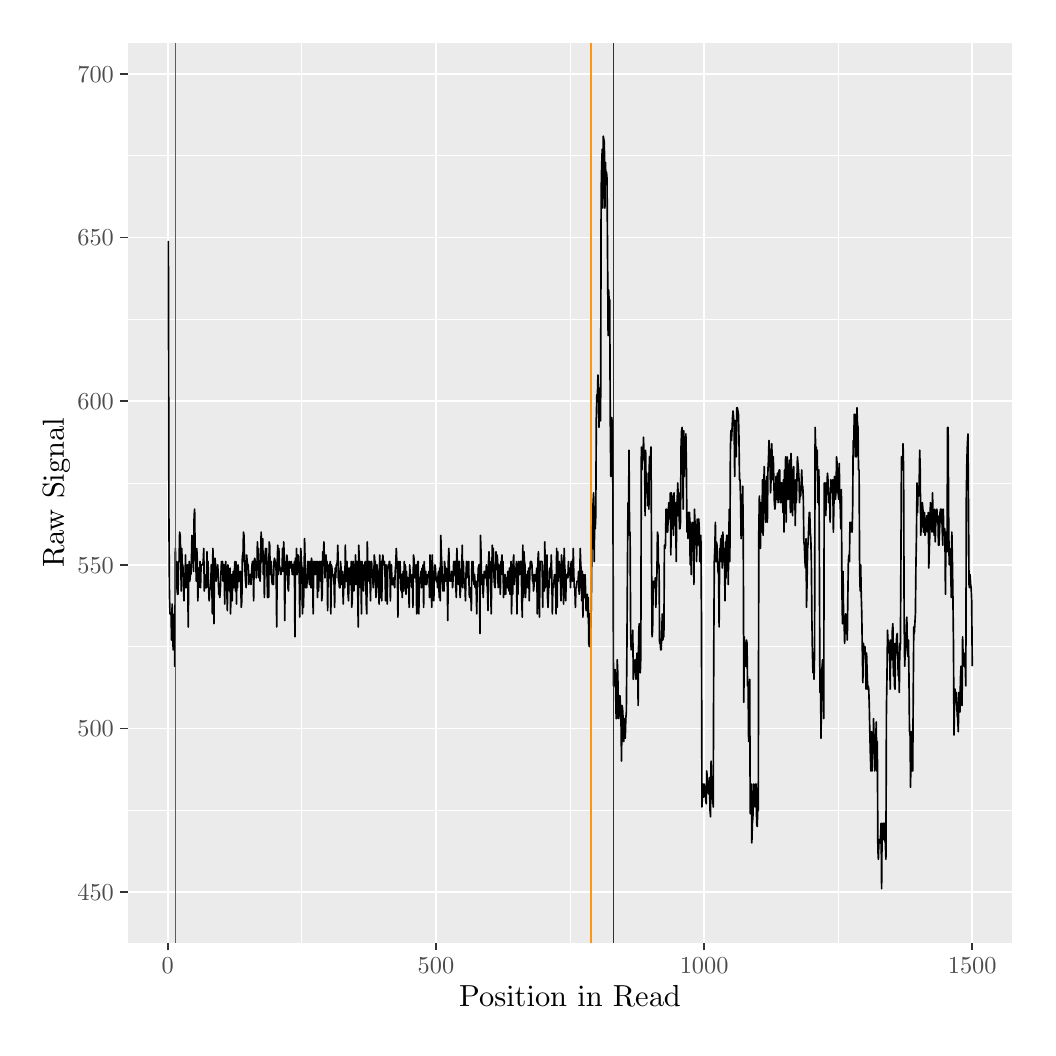
\begin{tikzpicture}[x=1pt,y=1pt]
\definecolor{fillColor}{RGB}{255,255,255}
\path[use as bounding box,fill=fillColor,fill opacity=0.00] (0,0) rectangle (361.35,361.35);
\begin{scope}
\path[clip] (  0.00,  0.00) rectangle (361.35,361.35);
\definecolor{drawColor}{RGB}{255,255,255}
\definecolor{fillColor}{RGB}{255,255,255}

\path[draw=drawColor,line width= 0.6pt,line join=round,line cap=round,fill=fillColor] (  0.00,  0.00) rectangle (361.35,361.35);
\end{scope}
\begin{scope}
\path[clip] ( 36.11, 30.69) rectangle (355.85,355.85);
\definecolor{fillColor}{gray}{0.92}

\path[fill=fillColor] ( 36.11, 30.69) rectangle (355.85,355.85);
\definecolor{drawColor}{RGB}{255,255,255}

\path[draw=drawColor,line width= 0.3pt,line join=round] ( 36.11, 78.57) --
	(355.85, 78.57);

\path[draw=drawColor,line width= 0.3pt,line join=round] ( 36.11,137.69) --
	(355.85,137.69);

\path[draw=drawColor,line width= 0.3pt,line join=round] ( 36.11,196.82) --
	(355.85,196.82);

\path[draw=drawColor,line width= 0.3pt,line join=round] ( 36.11,255.94) --
	(355.85,255.94);

\path[draw=drawColor,line width= 0.3pt,line join=round] ( 36.11,315.06) --
	(355.85,315.06);

\path[draw=drawColor,line width= 0.3pt,line join=round] ( 99.09, 30.69) --
	( 99.09,355.85);

\path[draw=drawColor,line width= 0.3pt,line join=round] (195.98, 30.69) --
	(195.98,355.85);

\path[draw=drawColor,line width= 0.3pt,line join=round] (292.87, 30.69) --
	(292.87,355.85);

\path[draw=drawColor,line width= 0.6pt,line join=round] ( 36.11, 49.01) --
	(355.85, 49.01);

\path[draw=drawColor,line width= 0.6pt,line join=round] ( 36.11,108.13) --
	(355.85,108.13);

\path[draw=drawColor,line width= 0.6pt,line join=round] ( 36.11,167.25) --
	(355.85,167.25);

\path[draw=drawColor,line width= 0.6pt,line join=round] ( 36.11,226.38) --
	(355.85,226.38);

\path[draw=drawColor,line width= 0.6pt,line join=round] ( 36.11,285.50) --
	(355.85,285.50);

\path[draw=drawColor,line width= 0.6pt,line join=round] ( 36.11,344.62) --
	(355.85,344.62);

\path[draw=drawColor,line width= 0.6pt,line join=round] ( 50.64, 30.69) --
	( 50.64,355.85);

\path[draw=drawColor,line width= 0.6pt,line join=round] (147.54, 30.69) --
	(147.54,355.85);

\path[draw=drawColor,line width= 0.6pt,line join=round] (244.43, 30.69) --
	(244.43,355.85);

\path[draw=drawColor,line width= 0.6pt,line join=round] (341.32, 30.69) --
	(341.32,355.85);
\definecolor{drawColor}{RGB}{0,0,0}

\path[draw=drawColor,line width= 0.6pt,line join=round] ( 50.84,284.31) --
	( 51.03,184.99) --
	( 51.23,156.61) --
	( 51.42,149.52) --
	( 51.61,149.52) --
	( 51.81,149.52) --
	( 52.00,140.06) --
	( 52.20,153.07) --
	( 52.39,142.42) --
	( 52.58,136.51) --
	( 52.78,144.79) --
	( 52.97,149.52) --
	( 53.16,130.60) --
	( 53.36,173.17) --
	( 53.55,164.89) --
	( 53.75,168.44) --
	( 53.94,158.98) --
	( 54.13,156.61) --
	( 54.33,156.61) --
	( 54.52,168.44) --
	( 54.71,168.44) --
	( 54.91,179.08) --
	( 55.10,177.90) --
	( 55.30,170.80) --
	( 55.49,157.80) --
	( 55.68,173.17) --
	( 55.88,166.07) --
	( 56.07,167.25) --
	( 56.26,162.53) --
	( 56.46,154.25) --
	( 56.65,163.71) --
	( 56.85,161.34) --
	( 57.04,170.80) --
	( 57.23,158.98) --
	( 57.43,160.16) --
	( 57.62,162.53) --
	( 57.81,167.25) --
	( 58.01,144.79) --
	( 58.20,164.89) --
	( 58.40,168.44) --
	( 58.59,161.34) --
	( 58.78,163.71) --
	( 58.98,163.71) --
	( 59.17,168.44) --
	( 59.36,177.90) --
	( 59.56,175.53) --
	( 59.75,170.80) --
	( 59.95,164.89) --
	( 60.14,184.99) --
	( 60.33,187.36) --
	( 60.53,170.80) --
	( 60.72,170.80) --
	( 60.92,161.34) --
	( 61.11,173.17) --
	( 61.30,168.44) --
	( 61.50,154.25) --
	( 61.69,166.07) --
	( 61.88,158.98) --
	( 62.08,162.53) --
	( 62.27,168.44) --
	( 62.47,158.98) --
	( 62.66,167.25) --
	( 62.85,167.25) --
	( 63.05,167.25) --
	( 63.24,167.25) --
	( 63.43,168.44) --
	( 63.63,173.17) --
	( 63.82,157.80) --
	( 64.02,163.71) --
	( 64.21,158.98) --
	( 64.40,158.98) --
	( 64.60,158.98) --
	( 64.79,171.98) --
	( 64.98,163.71) --
	( 65.18,168.44) --
	( 65.37,158.98) --
	( 65.57,154.25) --
	( 65.76,157.80) --
	( 65.95,158.98) --
	( 66.15,158.98) --
	( 66.34,167.25) --
	( 66.53,161.34) --
	( 66.73,149.52) --
	( 66.92,173.17) --
	( 67.12,166.07) --
	( 67.31,145.97) --
	( 67.50,168.44) --
	( 67.70,169.62) --
	( 67.89,167.25) --
	( 68.09,161.34) --
	( 68.28,163.71) --
	( 68.47,164.89) --
	( 68.67,167.25) --
	( 68.86,163.71) --
	( 69.05,156.61) --
	( 69.25,156.61) --
	( 69.44,155.43) --
	( 69.64,158.98) --
	( 69.83,163.71) --
	( 70.02,168.44) --
	( 70.22,166.07) --
	( 70.41,168.44) --
	( 70.60,161.34) --
	( 70.80,167.25) --
	( 70.99,167.25) --
	( 71.19,153.07) --
	( 71.38,163.71) --
	( 71.57,168.44) --
	( 71.77,163.71) --
	( 71.96,158.98) --
	( 72.15,150.70) --
	( 72.35,167.25) --
	( 72.54,164.89) --
	( 72.74,164.89) --
	( 72.93,157.80) --
	( 73.12,166.07) --
	( 73.32,149.52) --
	( 73.51,163.71) --
	( 73.70,163.71) --
	( 73.90,154.25) --
	( 74.09,162.53) --
	( 74.29,164.89) --
	( 74.48,158.98) --
	( 74.67,163.71) --
	( 74.87,168.44) --
	( 75.06,157.80) --
	( 75.25,168.44) --
	( 75.45,153.07) --
	( 75.64,166.07) --
	( 75.84,158.98) --
	( 76.03,167.25) --
	( 76.22,163.71) --
	( 76.42,161.34) --
	( 76.61,163.71) --
	( 76.81,164.89) --
	( 77.00,160.16) --
	( 77.19,151.88) --
	( 77.39,154.25) --
	( 77.58,170.80) --
	( 77.77,168.44) --
	( 77.97,179.08) --
	( 78.16,177.90) --
	( 78.36,169.62) --
	( 78.55,164.89) --
	( 78.74,161.34) --
	( 78.94,158.98) --
	( 79.13,170.80) --
	( 79.32,168.44) --
	( 79.52,167.25) --
	( 79.71,167.25) --
	( 79.91,160.16) --
	( 80.10,163.71) --
	( 80.29,163.71) --
	( 80.49,163.71) --
	( 80.68,160.16) --
	( 80.87,163.71) --
	( 81.07,167.25) --
	( 81.26,168.44) --
	( 81.46,168.44) --
	( 81.65,154.25) --
	( 81.84,168.44) --
	( 82.04,169.62) --
	( 82.23,168.44) --
	( 82.42,168.44) --
	( 82.62,162.53) --
	( 82.81,163.71) --
	( 83.01,175.53) --
	( 83.20,168.44) --
	( 83.39,173.17) --
	( 83.59,162.53) --
	( 83.78,163.71) --
	( 83.98,161.34) --
	( 84.17,166.07) --
	( 84.36,179.08) --
	( 84.56,168.44) --
	( 84.75,170.80) --
	( 84.94,176.71) --
	( 85.14,163.71) --
	( 85.33,170.80) --
	( 85.53,155.43) --
	( 85.72,167.25) --
	( 85.91,173.17) --
	( 86.11,168.44) --
	( 86.30,173.17) --
	( 86.49,163.71) --
	( 86.69,155.43) --
	( 86.88,168.44) --
	( 87.08,155.43) --
	( 87.27,175.53) --
	( 87.46,174.35) --
	( 87.66,163.71) --
	( 87.85,168.44) --
	( 88.04,168.44) --
	( 88.24,161.34) --
	( 88.43,160.16) --
	( 88.63,161.34) --
	( 88.82,160.16) --
	( 89.01,168.44) --
	( 89.21,169.62) --
	( 89.40,168.44) --
	( 89.59,167.25) --
	( 89.79,164.89) --
	( 89.98,144.79) --
	( 90.18,168.44) --
	( 90.37,174.35) --
	( 90.56,163.71) --
	( 90.76,173.17) --
	( 90.95,167.25) --
	( 91.15,166.07) --
	( 91.34,164.89) --
	( 91.53,163.71) --
	( 91.73,166.07) --
	( 91.92,166.07) --
	( 92.11,173.17) --
	( 92.31,164.89) --
	( 92.50,175.53) --
	( 92.70,170.80) --
	( 92.89,147.15) --
	( 93.08,164.89) --
	( 93.28,168.44) --
	( 93.47,163.71) --
	( 93.66,170.80) --
	( 93.86,168.44) --
	( 94.05,158.98) --
	( 94.25,157.80) --
	( 94.44,164.89) --
	( 94.63,168.44) --
	( 94.83,166.07) --
	( 95.02,167.25) --
	( 95.21,168.44) --
	( 95.41,167.25) --
	( 95.60,163.71) --
	( 95.80,167.25) --
	( 95.99,163.71) --
	( 96.18,164.89) --
	( 96.38,168.44) --
	( 96.57,141.24) --
	( 96.76,169.62) --
	( 96.96,163.71) --
	( 97.15,173.17) --
	( 97.35,163.71) --
	( 97.54,170.80) --
	( 97.73,170.80) --
	( 97.93,166.07) --
	( 98.12,163.71) --
	( 98.31,148.34) --
	( 98.51,167.25) --
	( 98.70,173.17) --
	( 98.90,168.44) --
	( 99.09,166.07) --
	( 99.28,149.52) --
	( 99.48,166.07) --
	( 99.67,151.88) --
	( 99.87,163.71) --
	(100.06,176.71) --
	(100.25,168.44) --
	(100.45,158.98) --
	(100.64,163.71) --
	(100.83,158.98) --
	(101.03,162.53) --
	(101.22,168.44) --
	(101.42,168.44) --
	(101.61,164.89) --
	(101.80,160.16) --
	(102.00,168.44) --
	(102.19,160.16) --
	(102.38,158.98) --
	(102.58,169.62) --
	(102.77,167.25) --
	(102.97,163.71) --
	(103.16,149.52) --
	(103.35,168.44) --
	(103.55,163.71) --
	(103.74,168.44) --
	(103.93,163.71) --
	(104.13,168.44) --
	(104.32,164.89) --
	(104.52,168.44) --
	(104.71,155.43) --
	(104.90,168.44) --
	(105.10,157.80) --
	(105.29,162.53) --
	(105.48,168.44) --
	(105.68,168.44) --
	(105.87,161.34) --
	(106.07,168.44) --
	(106.26,154.25) --
	(106.45,156.61) --
	(106.65,171.98) --
	(106.84,168.44) --
	(107.04,175.53) --
	(107.23,168.44) --
	(107.42,162.53) --
	(107.62,168.44) --
	(107.81,170.80) --
	(108.00,164.89) --
	(108.20,168.44) --
	(108.39,150.70) --
	(108.59,167.25) --
	(108.78,163.71) --
	(108.97,162.53) --
	(109.17,167.25) --
	(109.36,168.44) --
	(109.55,149.52) --
	(109.75,167.25) --
	(109.94,166.07) --
	(110.14,163.71) --
	(110.33,163.71) --
	(110.52,162.53) --
	(110.72,160.16) --
	(110.91,151.88) --
	(111.10,166.07) --
	(111.30,162.53) --
	(111.49,167.25) --
	(111.69,167.25) --
	(111.88,168.44) --
	(112.07,174.35) --
	(112.27,161.34) --
	(112.46,161.34) --
	(112.65,158.98) --
	(112.85,158.98) --
	(113.04,168.44) --
	(113.24,166.07) --
	(113.43,160.16) --
	(113.62,160.16) --
	(113.82,164.89) --
	(114.01,153.07) --
	(114.20,160.16) --
	(114.40,163.71) --
	(114.59,158.98) --
	(114.79,174.35) --
	(114.98,161.34) --
	(115.17,161.34) --
	(115.37,168.44) --
	(115.56,164.89) --
	(115.76,156.61) --
	(115.95,154.25) --
	(116.14,166.07) --
	(116.34,166.07) --
	(116.53,160.16) --
	(116.72,162.53) --
	(116.92,168.44) --
	(117.11,151.88) --
	(117.31,155.43) --
	(117.50,168.44) --
	(117.69,168.44) --
	(117.89,157.80) --
	(118.08,167.25) --
	(118.27,160.16) --
	(118.47,170.80) --
	(118.66,160.16) --
	(118.86,168.44) --
	(119.05,168.44) --
	(119.24,160.16) --
	(119.44,144.79) --
	(119.63,174.35) --
	(119.82,168.44) --
	(120.02,167.25) --
	(120.21,158.98) --
	(120.41,168.44) --
	(120.60,149.52) --
	(120.79,168.44) --
	(120.99,166.07) --
	(121.18,161.34) --
	(121.37,157.80) --
	(121.57,167.25) --
	(121.76,167.25) --
	(121.96,168.44) --
	(122.15,163.71) --
	(122.34,153.07) --
	(122.54,149.52) --
	(122.73,175.53) --
	(122.93,164.89) --
	(123.12,162.53) --
	(123.31,161.34) --
	(123.51,168.44) --
	(123.70,161.34) --
	(123.89,154.25) --
	(124.09,168.44) --
	(124.28,168.44) --
	(124.48,163.71) --
	(124.67,163.71) --
	(124.86,158.98) --
	(125.06,161.34) --
	(125.25,170.80) --
	(125.44,168.44) --
	(125.64,168.44) --
	(125.83,155.43) --
	(126.03,158.98) --
	(126.22,167.25) --
	(126.41,163.71) --
	(126.61,164.89) --
	(126.80,158.98) --
	(126.99,153.07) --
	(127.19,170.80) --
	(127.38,162.53) --
	(127.58,155.43) --
	(127.77,168.44) --
	(127.96,154.25) --
	(128.16,168.44) --
	(128.35,170.80) --
	(128.54,167.25) --
	(128.74,168.44) --
	(128.93,168.44) --
	(129.13,163.71) --
	(129.32,154.25) --
	(129.51,167.25) --
	(129.71,163.71) --
	(129.90,153.07) --
	(130.10,166.07) --
	(130.29,167.25) --
	(130.48,166.07) --
	(130.68,168.44) --
	(130.87,168.44) --
	(131.06,154.25) --
	(131.26,166.07) --
	(131.45,167.25) --
	(131.65,160.16) --
	(131.84,160.16) --
	(132.03,160.16) --
	(132.23,162.53) --
	(132.42,160.16) --
	(132.61,158.98) --
	(132.81,164.89) --
	(133.00,167.25) --
	(133.20,173.17) --
	(133.39,168.44) --
	(133.58,166.07) --
	(133.78,148.34) --
	(133.97,168.44) --
	(134.16,163.71) --
	(134.36,162.53) --
	(134.55,168.44) --
	(134.75,162.53) --
	(134.94,157.80) --
	(135.13,163.71) --
	(135.33,155.43) --
	(135.52,162.53) --
	(135.71,164.89) --
	(135.91,157.80) --
	(136.10,168.44) --
	(136.30,163.71) --
	(136.49,167.25) --
	(136.68,156.61) --
	(136.88,164.89) --
	(137.07,160.16) --
	(137.26,158.98) --
	(137.46,162.53) --
	(137.65,160.16) --
	(137.85,151.88) --
	(138.04,167.25) --
	(138.23,163.71) --
	(138.43,163.71) --
	(138.62,162.53) --
	(138.82,158.98) --
	(139.01,163.71) --
	(139.20,151.88) --
	(139.40,170.80) --
	(139.59,169.62) --
	(139.78,166.07) --
	(139.98,162.53) --
	(140.17,166.07) --
	(140.37,167.25) --
	(140.56,149.52) --
	(140.75,163.71) --
	(140.95,168.44) --
	(141.14,168.44) --
	(141.33,149.52) --
	(141.53,160.16) --
	(141.72,162.53) --
	(141.92,161.34) --
	(142.11,164.89) --
	(142.30,158.98) --
	(142.50,166.07) --
	(142.69,162.53) --
	(142.88,167.25) --
	(143.08,151.88) --
	(143.27,168.44) --
	(143.47,163.71) --
	(143.66,160.16) --
	(143.85,164.89) --
	(144.05,160.16) --
	(144.24,160.16) --
	(144.43,163.71) --
	(144.63,163.71) --
	(144.82,163.71) --
	(145.02,164.89) --
	(145.21,155.43) --
	(145.40,170.80) --
	(145.60,161.34) --
	(145.79,162.53) --
	(145.99,151.88) --
	(146.18,170.80) --
	(146.37,163.71) --
	(146.57,160.16) --
	(146.76,154.25) --
	(146.95,163.71) --
	(147.15,167.25) --
	(147.34,166.07) --
	(147.54,162.53) --
	(147.73,161.34) --
	(147.92,162.53) --
	(148.12,158.98) --
	(148.31,163.71) --
	(148.50,164.89) --
	(148.70,155.43) --
	(148.89,166.07) --
	(149.09,154.25) --
	(149.28,177.90) --
	(149.47,170.80) --
	(149.67,167.25) --
	(149.86,161.34) --
	(150.05,157.80) --
	(150.25,162.53) --
	(150.44,157.80) --
	(150.64,168.44) --
	(150.83,166.07) --
	(151.02,161.34) --
	(151.22,166.07) --
	(151.41,164.89) --
	(151.60,162.53) --
	(151.80,147.15) --
	(151.99,168.44) --
	(152.19,173.17) --
	(152.38,163.71) --
	(152.57,161.34) --
	(152.77,163.71) --
	(152.96,161.34) --
	(153.15,164.89) --
	(153.35,163.71) --
	(153.54,158.98) --
	(153.74,162.53) --
	(153.93,168.44) --
	(154.12,163.71) --
	(154.32,168.44) --
	(154.51,168.44) --
	(154.71,158.98) --
	(154.90,155.43) --
	(155.09,173.17) --
	(155.29,166.07) --
	(155.48,163.71) --
	(155.67,160.16) --
	(155.87,168.44) --
	(156.06,168.44) --
	(156.26,155.43) --
	(156.45,158.98) --
	(156.64,163.71) --
	(156.84,163.71) --
	(157.03,174.35) --
	(157.22,158.98) --
	(157.42,168.44) --
	(157.61,162.53) --
	(157.81,161.34) --
	(158.00,160.16) --
	(158.19,154.25) --
	(158.39,163.71) --
	(158.58,168.44) --
	(158.77,168.44) --
	(158.97,163.71) --
	(159.16,162.53) --
	(159.36,168.44) --
	(159.55,156.61) --
	(159.74,155.43) --
	(159.94,158.98) --
	(160.13,156.61) --
	(160.32,150.70) --
	(160.52,168.44) --
	(160.71,167.25) --
	(160.91,168.44) --
	(161.10,163.71) --
	(161.29,160.16) --
	(161.49,163.71) --
	(161.68,158.98) --
	(161.88,161.34) --
	(162.07,158.98) --
	(162.26,149.52) --
	(162.46,161.34) --
	(162.65,161.34) --
	(162.84,166.07) --
	(163.04,167.25) --
	(163.23,167.25) --
	(163.43,142.42) --
	(163.62,177.90) --
	(163.81,171.98) --
	(164.01,160.16) --
	(164.20,163.71) --
	(164.39,163.71) --
	(164.59,155.43) --
	(164.78,160.16) --
	(164.98,164.89) --
	(165.17,164.89) --
	(165.36,162.53) --
	(165.56,162.53) --
	(165.75,167.25) --
	(165.94,160.16) --
	(166.14,158.98) --
	(166.33,150.70) --
	(166.53,168.44) --
	(166.72,171.98) --
	(166.91,162.53) --
	(167.11,168.44) --
	(167.30,161.34) --
	(167.49,149.52) --
	(167.69,162.53) --
	(167.88,174.35) --
	(168.08,166.07) --
	(168.27,173.17) --
	(168.46,163.71) --
	(168.66,160.16) --
	(168.85,158.98) --
	(169.05,162.53) --
	(169.24,171.98) --
	(169.43,168.44) --
	(169.63,170.80) --
	(169.82,168.44) --
	(170.01,158.98) --
	(170.21,167.25) --
	(170.40,163.71) --
	(170.60,163.71) --
	(170.79,156.61) --
	(170.98,168.44) --
	(171.18,166.07) --
	(171.37,170.80) --
	(171.56,163.71) --
	(171.76,168.44) --
	(171.95,155.43) --
	(172.15,158.98) --
	(172.34,156.61) --
	(172.53,163.71) --
	(172.73,156.61) --
	(172.92,162.53) --
	(173.11,162.53) --
	(173.31,158.98) --
	(173.50,164.89) --
	(173.70,161.34) --
	(173.89,157.80) --
	(174.08,166.07) --
	(174.28,156.61) --
	(174.47,163.71) --
	(174.66,168.44) --
	(174.86,149.52) --
	(175.05,167.25) --
	(175.25,156.61) --
	(175.44,168.44) --
	(175.63,170.80) --
	(175.83,160.16) --
	(176.02,163.71) --
	(176.21,166.07) --
	(176.41,163.71) --
	(176.60,168.44) --
	(176.80,149.52) --
	(176.99,166.07) --
	(177.18,156.61) --
	(177.38,168.44) --
	(177.57,164.89) --
	(177.77,163.71) --
	(177.96,168.44) --
	(178.15,168.44) --
	(178.35,168.44) --
	(178.54,154.25) --
	(178.73,148.34) --
	(178.93,174.35) --
	(179.12,155.43) --
	(179.32,171.98) --
	(179.51,168.44) --
	(179.70,167.25) --
	(179.90,155.43) --
	(180.09,161.34) --
	(180.28,163.71) --
	(180.48,158.98) --
	(180.67,164.89) --
	(180.87,163.71) --
	(181.06,166.07) --
	(181.25,154.25) --
	(181.45,164.89) --
	(181.64,168.44) --
	(181.83,168.44) --
	(182.03,168.44) --
	(182.22,167.25) --
	(182.42,161.34) --
	(182.61,163.71) --
	(182.80,157.80) --
	(183.00,160.16) --
	(183.19,163.71) --
	(183.38,161.34) --
	(183.58,162.53) --
	(183.77,163.71) --
	(183.97,166.07) --
	(184.16,149.52) --
	(184.35,168.44) --
	(184.55,171.98) --
	(184.74,158.98) --
	(184.94,148.34) --
	(185.13,168.44) --
	(185.32,168.44) --
	(185.52,168.44) --
	(185.71,168.44) --
	(185.90,168.44) --
	(186.10,151.88) --
	(186.29,164.89) --
	(186.49,161.34) --
	(186.68,157.80) --
	(186.87,175.53) --
	(187.07,158.98) --
	(187.26,162.53) --
	(187.45,167.25) --
	(187.65,170.80) --
	(187.84,155.43) --
	(188.04,151.88) --
	(188.23,158.98) --
	(188.42,158.98) --
	(188.62,166.07) --
	(188.81,163.71) --
	(189.00,162.53) --
	(189.20,170.80) --
	(189.39,163.71) --
	(189.59,149.52) --
	(189.78,160.16) --
	(189.97,158.98) --
	(190.17,161.34) --
	(190.36,163.71) --
	(190.55,163.71) --
	(190.75,161.34) --
	(190.94,149.52) --
	(191.14,173.17) --
	(191.33,151.88) --
	(191.52,171.98) --
	(191.72,161.34) --
	(191.91,164.89) --
	(192.10,168.44) --
	(192.30,164.89) --
	(192.49,163.71) --
	(192.69,154.25) --
	(192.88,170.80) --
	(193.07,168.44) --
	(193.27,164.89) --
	(193.46,158.98) --
	(193.66,153.07) --
	(193.85,173.17) --
	(194.04,167.25) --
	(194.24,163.71) --
	(194.43,154.25) --
	(194.62,163.71) --
	(194.82,163.71) --
	(195.01,163.71) --
	(195.21,162.53) --
	(195.40,168.44) --
	(195.59,163.71) --
	(195.79,166.07) --
	(195.98,163.71) --
	(196.17,158.98) --
	(196.37,168.44) --
	(196.56,168.44) --
	(196.76,166.07) --
	(196.95,161.34) --
	(197.14,173.17) --
	(197.34,163.71) --
	(197.53,158.98) --
	(197.72,158.98) --
	(197.92,151.88) --
	(198.11,158.98) --
	(198.31,158.98) --
	(198.50,161.34) --
	(198.69,161.34) --
	(198.89,161.34) --
	(199.08,164.89) --
	(199.27,156.61) --
	(199.47,158.98) --
	(199.66,173.17) --
	(199.86,167.25) --
	(200.05,164.89) --
	(200.24,154.25) --
	(200.44,164.89) --
	(200.63,148.34) --
	(200.83,163.71) --
	(201.02,158.98) --
	(201.21,155.43) --
	(201.41,163.71) --
	(201.60,157.80) --
	(201.79,150.70) --
	(201.99,155.43) --
	(202.18,156.61) --
	(202.38,148.34) --
	(202.57,155.43) --
	(202.76,138.88) --
	(202.96,137.69) --
	(203.15,149.52) --
	(203.34,149.52) --
	(203.54,144.79) --
	(203.73,158.98) --
	(203.93,181.44) --
	(204.12,173.17) --
	(204.31,189.72) --
	(204.51,193.27) --
	(204.70,168.44) --
	(204.89,184.99) --
	(205.09,180.26) --
	(205.28,184.99) --
	(205.48,220.46) --
	(205.67,228.74) --
	(205.86,227.56) --
	(206.06,235.83) --
	(206.25,228.74) --
	(206.44,216.92) --
	(206.64,231.11) --
	(206.83,231.11) --
	(207.03,219.28) --
	(207.22,302.05) --
	(207.41,311.51) --
	(207.61,317.42) --
	(207.80,296.14) --
	(208.00,322.15) --
	(208.19,320.97) --
	(208.38,319.79) --
	(208.58,296.14) --
	(208.77,312.69) --
	(208.96,306.78) --
	(209.16,309.14) --
	(209.35,306.78) --
	(209.55,277.22) --
	(209.74,250.02) --
	(209.93,266.58) --
	(210.13,261.85) --
	(210.32,263.03) --
	(210.51,220.46) --
	(210.71,199.18) --
	(210.90,219.28) --
	(211.10,220.46) --
	(211.29,212.19) --
	(211.48,193.27) --
	(211.68,123.51) --
	(211.87,128.24) --
	(212.06,123.51) --
	(212.26,129.42) --
	(212.45,122.32) --
	(212.65,111.68) --
	(212.84,111.68) --
	(213.03,132.96) --
	(213.23,128.24) --
	(213.42,117.59) --
	(213.61,111.68) --
	(213.81,115.23) --
	(214.00,119.96) --
	(214.20,116.41) --
	(214.39,111.68) --
	(214.58, 96.31) --
	(214.78,116.41) --
	(214.97,115.23) --
	(215.16,111.68) --
	(215.36,103.40) --
	(215.55,111.68) --
	(215.75,105.77) --
	(215.94,104.59) --
	(216.13,111.68) --
	(216.33,114.05) --
	(216.52,135.33) --
	(216.72,164.89) --
	(216.91,189.72) --
	(217.10,183.81) --
	(217.30,208.64) --
	(217.49,177.90) --
	(217.68,179.08) --
	(217.88,142.42) --
	(218.07,136.51) --
	(218.27,141.24) --
	(218.46,138.88) --
	(218.65,143.61) --
	(218.85,125.87) --
	(219.04,129.42) --
	(219.23,130.60) --
	(219.43,132.96) --
	(219.62,130.60) --
	(219.82,125.87) --
	(220.01,131.78) --
	(220.20,135.33) --
	(220.40,135.33) --
	(220.59,116.41) --
	(220.78,142.42) --
	(220.98,145.97) --
	(221.17,135.33) --
	(221.37,128.24) --
	(221.56,134.15) --
	(221.75,209.82) --
	(221.95,201.54) --
	(222.14,206.27) --
	(222.33,205.09) --
	(222.53,213.37) --
	(222.72,206.27) --
	(222.92,205.09) --
	(223.11,184.99) --
	(223.30,208.64) --
	(223.50,193.27) --
	(223.69,196.82) --
	(223.89,195.63) --
	(224.08,188.54) --
	(224.27,200.36) --
	(224.47,187.36) --
	(224.66,206.27) --
	(224.85,199.18) --
	(225.05,206.27) --
	(225.24,209.82) --
	(225.44,168.44) --
	(225.63,141.24) --
	(225.82,143.61) --
	(226.02,160.16) --
	(226.21,161.34) --
	(226.40,158.98) --
	(226.60,160.16) --
	(226.79,162.53) --
	(226.99,151.88) --
	(227.18,158.98) --
	(227.37,163.71) --
	(227.57,179.08) --
	(227.76,177.90) --
	(227.95,166.07) --
	(228.15,167.25) --
	(228.34,138.88) --
	(228.54,140.06) --
	(228.73,136.51) --
	(228.92,136.51) --
	(229.12,142.42) --
	(229.31,149.52) --
	(229.50,140.06) --
	(229.70,141.24) --
	(229.89,141.24) --
	(230.09,174.35) --
	(230.28,173.17) --
	(230.47,174.35) --
	(230.67,187.36) --
	(230.86,187.36) --
	(231.05,181.44) --
	(231.25,179.08) --
	(231.44,183.81) --
	(231.64,189.72) --
	(231.83,184.99) --
	(232.02,183.81) --
	(232.22,193.27) --
	(232.41,170.80) --
	(232.61,193.27) --
	(232.80,180.26) --
	(232.99,189.72) --
	(233.19,192.09) --
	(233.38,177.90) --
	(233.57,193.27) --
	(233.77,181.44) --
	(233.96,189.72) --
	(234.16,186.17) --
	(234.35,168.44) --
	(234.54,187.36) --
	(234.74,192.09) --
	(234.93,196.82) --
	(235.12,184.99) --
	(235.32,193.27) --
	(235.51,180.26) --
	(235.71,180.26) --
	(235.90,182.63) --
	(236.09,209.82) --
	(236.29,215.73) --
	(236.48,216.92) --
	(236.67,206.27) --
	(236.87,187.36) --
	(237.06,215.73) --
	(237.26,199.18) --
	(237.45,208.64) --
	(237.64,206.27) --
	(237.84,214.55) --
	(238.03,202.73) --
	(238.22,179.08) --
	(238.42,183.81) --
	(238.61,176.71) --
	(238.81,186.17) --
	(239.00,186.17) --
	(239.19,186.17) --
	(239.39,167.25) --
	(239.58,182.63) --
	(239.78,163.71) --
	(239.97,179.08) --
	(240.16,174.35) --
	(240.36,182.63) --
	(240.55,179.08) --
	(240.74,160.16) --
	(240.94,187.36) --
	(241.13,182.63) --
	(241.33,180.26) --
	(241.52,180.26) --
	(241.71,168.44) --
	(241.91,183.81) --
	(242.10,174.35) --
	(242.29,179.08) --
	(242.49,183.81) --
	(242.68,180.26) --
	(242.88,168.44) --
	(243.07,175.53) --
	(243.26,177.90) --
	(243.46,149.52) --
	(243.65, 79.76) --
	(243.84, 84.49) --
	(244.04, 88.03) --
	(244.23, 83.30) --
	(244.43, 88.03) --
	(244.62, 86.85) --
	(244.81, 86.85) --
	(245.01, 82.12) --
	(245.20, 80.94) --
	(245.39, 92.76) --
	(245.59, 89.22) --
	(245.78, 88.03) --
	(245.98, 84.49) --
	(246.17, 85.67) --
	(246.36, 90.40) --
	(246.56, 78.57) --
	(246.75, 76.21) --
	(246.95, 96.31) --
	(247.14, 86.85) --
	(247.33, 84.49) --
	(247.53, 83.30) --
	(247.72, 79.76) --
	(247.91,135.33) --
	(248.11,168.44) --
	(248.30,173.17) --
	(248.50,182.63) --
	(248.69,168.44) --
	(248.88,175.53) --
	(249.08,174.35) --
	(249.27,168.44) --
	(249.46,164.89) --
	(249.66,163.71) --
	(249.85,144.79) --
	(250.05,173.17) --
	(250.24,168.44) --
	(250.43,176.71) --
	(250.63,168.44) --
	(250.82,177.90) --
	(251.01,166.07) --
	(251.21,179.08) --
	(251.40,168.44) --
	(251.60,173.17) --
	(251.79,169.62) --
	(251.98,154.25) --
	(252.18,175.53) --
	(252.37,162.53) --
	(252.56,177.90) --
	(252.76,173.17) --
	(252.95,177.90) --
	(253.15,160.16) --
	(253.34,176.71) --
	(253.53,187.36) --
	(253.73,168.44) --
	(253.92,208.64) --
	(254.11,215.73) --
	(254.31,212.19) --
	(254.50,215.73) --
	(254.70,220.46) --
	(254.89,222.83) --
	(255.08,220.46) --
	(255.28,216.92) --
	(255.47,199.18) --
	(255.67,219.28) --
	(255.86,219.28) --
	(256.05,206.27) --
	(256.25,224.01) --
	(256.44,224.01) --
	(256.63,222.83) --
	(256.83,221.65) --
	(257.02,213.37) --
	(257.22,198.00) --
	(257.41,198.00) --
	(257.60,190.90) --
	(257.80,176.71) --
	(257.99,187.36) --
	(258.18,184.99) --
	(258.38,195.63) --
	(258.57,177.90) --
	(258.77,117.59) --
	(258.96,141.24) --
	(259.15,130.60) --
	(259.35,130.60) --
	(259.54,130.60) --
	(259.73,140.06) --
	(259.93,138.88) --
	(260.12,123.51) --
	(260.32,124.69) --
	(260.51,103.40) --
	(260.70,122.32) --
	(260.90,125.87) --
	(261.09, 77.39) --
	(261.28, 78.57) --
	(261.48, 88.03) --
	(261.67, 66.75) --
	(261.87, 73.84) --
	(262.06, 76.21) --
	(262.25, 88.03) --
	(262.45, 79.76) --
	(262.64, 83.30) --
	(262.84, 88.03) --
	(263.03, 79.76) --
	(263.22, 88.03) --
	(263.42, 73.84) --
	(263.61, 72.66) --
	(263.80, 78.57) --
	(264.00, 78.57) --
	(264.19,179.08) --
	(264.39,192.09) --
	(264.58,182.63) --
	(264.77,173.17) --
	(264.97,189.72) --
	(265.16,179.08) --
	(265.35,184.99) --
	(265.55,198.00) --
	(265.74,177.90) --
	(265.94,187.36) --
	(266.13,202.73) --
	(266.32,192.09) --
	(266.52,190.90) --
	(266.71,182.63) --
	(266.90,196.82) --
	(267.10,199.18) --
	(267.29,182.63) --
	(267.49,201.54) --
	(267.68,205.09) --
	(267.87,212.19) --
	(268.07,208.64) --
	(268.26,202.73) --
	(268.45,193.27) --
	(268.65,199.18) --
	(268.84,211.00) --
	(269.04,206.27) --
	(269.23,198.00) --
	(269.42,206.27) --
	(269.62,198.00) --
	(269.81,189.72) --
	(270.00,187.36) --
	(270.20,189.72) --
	(270.39,199.18) --
	(270.59,199.18) --
	(270.78,190.90) --
	(270.97,200.36) --
	(271.17,189.72) --
	(271.36,200.36) --
	(271.56,201.54) --
	(271.75,201.54) --
	(271.94,189.72) --
	(272.14,189.72) --
	(272.33,196.82) --
	(272.52,196.82) --
	(272.72,195.63) --
	(272.91,186.17) --
	(273.11,198.00) --
	(273.30,179.08) --
	(273.49,201.54) --
	(273.69,196.82) --
	(273.88,206.27) --
	(274.07,182.63) --
	(274.27,198.00) --
	(274.46,206.27) --
	(274.66,196.82) --
	(274.85,190.90) --
	(275.04,193.27) --
	(275.24,205.09) --
	(275.43,193.27) --
	(275.62,186.17) --
	(275.82,207.46) --
	(276.01,201.54) --
	(276.21,201.54) --
	(276.40,184.99) --
	(276.59,198.00) --
	(276.79,202.73) --
	(276.98,189.72) --
	(277.17,196.82) --
	(277.37,181.44) --
	(277.56,198.00) --
	(277.76,189.72) --
	(277.95,196.82) --
	(278.14,206.27) --
	(278.34,203.91) --
	(278.53,201.54) --
	(278.73,198.00) --
	(278.92,189.72) --
	(279.11,195.63) --
	(279.31,192.09) --
	(279.50,195.63) --
	(279.69,201.54) --
	(279.89,195.63) --
	(280.08,195.63) --
	(280.28,190.90) --
	(280.47,175.53) --
	(280.66,174.35) --
	(280.86,168.44) --
	(281.05,166.07) --
	(281.24,176.71) --
	(281.44,151.88) --
	(281.63,161.34) --
	(281.83,173.17) --
	(282.02,175.53) --
	(282.21,180.26) --
	(282.41,186.17) --
	(282.60,186.17) --
	(282.79,179.08) --
	(282.99,176.71) --
	(283.18,168.44) --
	(283.38,147.15) --
	(283.57,135.33) --
	(283.76,128.24) --
	(283.96,134.15) --
	(284.15,125.87) --
	(284.34,135.33) --
	(284.54,216.92) --
	(284.73,209.82) --
	(284.93,209.82) --
	(285.12,201.54) --
	(285.31,208.64) --
	(285.51,189.72) --
	(285.70,198.00) --
	(285.90,201.54) --
	(286.09,167.25) --
	(286.28,121.14) --
	(286.48,129.42) --
	(286.67,104.59) --
	(286.86,122.32) --
	(287.06,130.60) --
	(287.25,132.96) --
	(287.45,122.32) --
	(287.64,111.68) --
	(287.83,196.82) --
	(288.03,187.36) --
	(288.22,196.82) --
	(288.41,184.99) --
	(288.61,196.82) --
	(288.80,195.63) --
	(289.00,200.36) --
	(289.19,198.00) --
	(289.38,189.72) --
	(289.58,193.27) --
	(289.77,192.09) --
	(289.96,182.63) --
	(290.16,198.00) --
	(290.35,193.27) --
	(290.55,196.82) --
	(290.74,196.82) --
	(290.93,198.00) --
	(291.13,179.08) --
	(291.32,188.54) --
	(291.51,199.18) --
	(291.71,192.09) --
	(291.90,190.90) --
	(292.10,194.45) --
	(292.29,206.27) --
	(292.48,203.91) --
	(292.68,193.27) --
	(292.87,193.27) --
	(293.06,190.90) --
	(293.26,203.91) --
	(293.45,192.09) --
	(293.65,187.36) --
	(293.84,180.26) --
	(294.03,194.45) --
	(294.23,157.80) --
	(294.42,145.97) --
	(294.62,164.89) --
	(294.81,149.52) --
	(295.00,147.15) --
	(295.20,138.88) --
	(295.39,144.79) --
	(295.58,149.52) --
	(295.78,147.15) --
	(295.97,144.79) --
	(296.17,140.06) --
	(296.36,155.43) --
	(296.55,168.44) --
	(296.75,170.80) --
	(296.94,168.44) --
	(297.13,182.63) --
	(297.33,179.08) --
	(297.52,180.26) --
	(297.72,182.63) --
	(297.91,179.08) --
	(298.10,187.36) --
	(298.30,212.19) --
	(298.49,209.82) --
	(298.68,221.65) --
	(298.88,216.92) --
	(299.07,206.27) --
	(299.27,221.65) --
	(299.46,206.27) --
	(299.65,224.01) --
	(299.85,218.10) --
	(300.04,216.92) --
	(300.23,201.54) --
	(300.43,201.54) --
	(300.62,166.07) --
	(300.82,157.80) --
	(301.01,167.25) --
	(301.20,156.61) --
	(301.40,149.52) --
	(301.59,136.51) --
	(301.79,124.69) --
	(301.98,138.88) --
	(302.17,136.51) --
	(302.37,137.69) --
	(302.56,137.69) --
	(302.75,132.96) --
	(302.95,122.32) --
	(303.14,135.33) --
	(303.34,128.24) --
	(303.53,122.32) --
	(303.72,123.51) --
	(303.92,122.32) --
	(304.11,116.41) --
	(304.30,106.95) --
	(304.50, 98.67) --
	(304.69, 92.76) --
	(304.89,106.95) --
	(305.08, 92.76) --
	(305.27,103.40) --
	(305.47,101.04) --
	(305.66,111.68) --
	(305.85,103.40) --
	(306.05, 92.76) --
	(306.24,101.04) --
	(306.44,103.40) --
	(306.63,110.50) --
	(306.82, 92.76) --
	(307.02,103.40) --
	(307.21, 64.38) --
	(307.40, 60.84) --
	(307.60, 67.93) --
	(307.79, 67.93) --
	(307.99, 66.75) --
	(308.18, 69.11) --
	(308.37, 73.84) --
	(308.57, 50.20) --
	(308.76, 73.84) --
	(308.95, 69.11) --
	(309.15, 67.93) --
	(309.34, 73.84) --
	(309.54, 73.84) --
	(309.73, 67.93) --
	(309.92, 66.75) --
	(310.12, 60.84) --
	(310.31,115.23) --
	(310.51,127.05) --
	(310.70,143.61) --
	(310.89,138.88) --
	(311.09,140.06) --
	(311.28,135.33) --
	(311.47,136.51) --
	(311.67,122.32) --
	(311.86,140.06) --
	(312.06,138.88) --
	(312.25,132.96) --
	(312.44,143.61) --
	(312.64,145.97) --
	(312.83,127.05) --
	(313.02,138.88) --
	(313.22,123.51) --
	(313.41,122.32) --
	(313.61,138.88) --
	(313.80,135.33) --
	(313.99,141.24) --
	(314.19,142.42) --
	(314.38,135.33) --
	(314.57,127.05) --
	(314.77,130.60) --
	(314.96,121.14) --
	(315.16,138.88) --
	(315.35,136.51) --
	(315.54,168.44) --
	(315.74,206.27) --
	(315.93,206.27) --
	(316.12,201.54) --
	(316.32,211.00) --
	(316.51,201.54) --
	(316.71,148.34) --
	(316.90,130.60) --
	(317.09,135.33) --
	(317.29,140.06) --
	(317.48,142.42) --
	(317.68,148.34) --
	(317.87,137.69) --
	(318.06,134.15) --
	(318.26,140.06) --
	(318.45,127.05) --
	(318.64,106.95) --
	(318.84,106.95) --
	(319.03, 86.85) --
	(319.23,106.95) --
	(319.42, 92.76) --
	(319.61, 98.67) --
	(319.81, 92.76) --
	(320.00,121.14) --
	(320.19,144.79) --
	(320.39,142.42) --
	(320.58,145.97) --
	(320.78,149.52) --
	(320.97,167.25) --
	(321.16,177.90) --
	(321.36,196.82) --
	(321.55,186.17) --
	(321.74,195.63) --
	(321.94,192.09) --
	(322.13,195.63) --
	(322.33,208.64) --
	(322.52,201.54) --
	(322.71,177.90) --
	(322.91,181.44) --
	(323.10,182.63) --
	(323.29,189.72) --
	(323.49,187.36) --
	(323.68,179.08) --
	(323.88,180.26) --
	(324.07,186.17) --
	(324.26,177.90) --
	(324.46,179.08) --
	(324.65,180.26) --
	(324.85,184.99) --
	(325.04,181.44) --
	(325.23,179.08) --
	(325.43,186.17) --
	(325.62,166.07) --
	(325.81,173.17) --
	(326.01,179.08) --
	(326.20,189.72) --
	(326.40,187.36) --
	(326.59,182.63) --
	(326.78,179.08) --
	(326.98,193.27) --
	(327.17,180.26) --
	(327.36,182.63) --
	(327.56,177.90) --
	(327.75,187.36) --
	(327.95,175.53) --
	(328.14,182.63) --
	(328.33,182.63) --
	(328.53,187.36) --
	(328.72,183.81) --
	(328.91,184.99) --
	(329.11,174.35) --
	(329.30,174.35) --
	(329.50,179.08) --
	(329.69,186.17) --
	(329.88,187.36) --
	(330.08,182.63) --
	(330.27,187.36) --
	(330.46,180.26) --
	(330.66,174.35) --
	(330.85,187.36) --
	(331.05,177.90) --
	(331.24,180.26) --
	(331.43,180.26) --
	(331.63,156.61) --
	(331.82,179.08) --
	(332.01,176.71) --
	(332.21,171.98) --
	(332.40,216.92) --
	(332.60,216.92) --
	(332.79,184.99) --
	(332.98,167.25) --
	(333.18,173.17) --
	(333.37,171.98) --
	(333.57,163.71) --
	(333.76,155.43) --
	(333.95,179.08) --
	(334.15,168.44) --
	(334.34,155.43) --
	(334.53,138.88) --
	(334.73,105.77) --
	(334.92,117.59) --
	(335.12,122.32) --
	(335.31,117.59) --
	(335.50,121.14) --
	(335.70,117.59) --
	(335.89,112.86) --
	(336.08,111.68) --
	(336.28,106.95) --
	(336.47,121.14) --
	(336.67,118.78) --
	(336.86,114.05) --
	(337.05,125.87) --
	(337.25,130.60) --
	(337.44,122.32) --
	(337.63,116.41) --
	(337.83,141.24) --
	(338.02,134.15) --
	(338.22,134.15) --
	(338.41,130.60) --
	(338.60,135.33) --
	(338.80,130.60) --
	(338.99,123.51) --
	(339.18,192.09) --
	(339.38,205.09) --
	(339.57,211.00) --
	(339.77,214.55) --
	(339.96,187.36) --
	(340.15,160.16) --
	(340.35,158.98) --
	(340.54,163.71) --
	(340.74,160.16) --
	(340.93,158.98) --
	(341.12,154.25) --
	(341.32,130.60);
\definecolor{drawColor}{RGB}{255,0,0}

\path[draw=drawColor,draw opacity=0.90,line width= 0.6pt,line join=round] ( 53.36, 30.69) -- ( 53.36,355.85);
\definecolor{drawColor}{RGB}{255,140,0}

\path[draw=drawColor,draw opacity=0.90,line width= 0.6pt,line join=round] (203.54, 30.69) -- (203.54,355.85);
\definecolor{drawColor}{RGB}{0,0,255}

\path[draw=drawColor,draw opacity=0.90,line width= 0.6pt,line join=round] (211.68, 30.69) -- (211.68,355.85);
\end{scope}
\begin{scope}
\path[clip] (  0.00,  0.00) rectangle (361.35,361.35);
\definecolor{drawColor}{gray}{0.30}

\node[text=drawColor,anchor=base east,inner sep=0pt, outer sep=0pt, scale=  0.88] at ( 31.16, 45.98) {450};

\node[text=drawColor,anchor=base east,inner sep=0pt, outer sep=0pt, scale=  0.88] at ( 31.16,105.10) {500};

\node[text=drawColor,anchor=base east,inner sep=0pt, outer sep=0pt, scale=  0.88] at ( 31.16,164.22) {550};

\node[text=drawColor,anchor=base east,inner sep=0pt, outer sep=0pt, scale=  0.88] at ( 31.16,223.35) {600};

\node[text=drawColor,anchor=base east,inner sep=0pt, outer sep=0pt, scale=  0.88] at ( 31.16,282.47) {650};

\node[text=drawColor,anchor=base east,inner sep=0pt, outer sep=0pt, scale=  0.88] at ( 31.16,341.59) {700};
\end{scope}
\begin{scope}
\path[clip] (  0.00,  0.00) rectangle (361.35,361.35);
\definecolor{drawColor}{gray}{0.20}

\path[draw=drawColor,line width= 0.6pt,line join=round] ( 33.36, 49.01) --
	( 36.11, 49.01);

\path[draw=drawColor,line width= 0.6pt,line join=round] ( 33.36,108.13) --
	( 36.11,108.13);

\path[draw=drawColor,line width= 0.6pt,line join=round] ( 33.36,167.25) --
	( 36.11,167.25);

\path[draw=drawColor,line width= 0.6pt,line join=round] ( 33.36,226.38) --
	( 36.11,226.38);

\path[draw=drawColor,line width= 0.6pt,line join=round] ( 33.36,285.50) --
	( 36.11,285.50);

\path[draw=drawColor,line width= 0.6pt,line join=round] ( 33.36,344.62) --
	( 36.11,344.62);
\end{scope}
\begin{scope}
\path[clip] (  0.00,  0.00) rectangle (361.35,361.35);
\definecolor{drawColor}{gray}{0.20}

\path[draw=drawColor,line width= 0.6pt,line join=round] ( 50.64, 27.94) --
	( 50.64, 30.69);

\path[draw=drawColor,line width= 0.6pt,line join=round] (147.54, 27.94) --
	(147.54, 30.69);

\path[draw=drawColor,line width= 0.6pt,line join=round] (244.43, 27.94) --
	(244.43, 30.69);

\path[draw=drawColor,line width= 0.6pt,line join=round] (341.32, 27.94) --
	(341.32, 30.69);
\end{scope}
\begin{scope}
\path[clip] (  0.00,  0.00) rectangle (361.35,361.35);
\definecolor{drawColor}{gray}{0.30}

\node[text=drawColor,anchor=base,inner sep=0pt, outer sep=0pt, scale=  0.88] at ( 50.64, 19.68) {0};

\node[text=drawColor,anchor=base,inner sep=0pt, outer sep=0pt, scale=  0.88] at (147.54, 19.68) {500};

\node[text=drawColor,anchor=base,inner sep=0pt, outer sep=0pt, scale=  0.88] at (244.43, 19.68) {1000};

\node[text=drawColor,anchor=base,inner sep=0pt, outer sep=0pt, scale=  0.88] at (341.32, 19.68) {1500};
\end{scope}
\begin{scope}
\path[clip] (  0.00,  0.00) rectangle (361.35,361.35);
\definecolor{drawColor}{RGB}{0,0,0}

\node[text=drawColor,anchor=base,inner sep=0pt, outer sep=0pt, scale=  1.10] at (195.98,  7.64) {Position in Read};
\end{scope}
\begin{scope}
\path[clip] (  0.00,  0.00) rectangle (361.35,361.35);
\definecolor{drawColor}{RGB}{0,0,0}

\node[text=drawColor,rotate= 90.00,anchor=base,inner sep=0pt, outer sep=0pt, scale=  1.10] at ( 13.08,193.27) {Raw Signal};
\end{scope}
\end{tikzpicture}

	\caption[The first 1500 data points of the read with ID e9f08690-171f-476f-9119-5330d0290126 split into four sections: surge, stall, pre-adapter surge and adapter sequence.]{\label{fig:start-sections}The first 1500 data points of the read with ID e9f08690-171f-476f-9119-5330d0290126 split into four sections: surge (before the red line), stall (between red and orange), pre-adapter surge (between orange and blue) and adapter sequence (after blue). In order from left to right the vertical lines are coloured red, orange and blue.}
\end{figure}


The DNA sections are the sections of the signal data which store information necessary for determining the original DNA sequence. Characteristically, these oscillate in smaller low-variance sections of 10-100 signals with steep transitions between them. The adapter sequence is quite similar in behaviour since it also represents molecular information.

The homopolymer and stuck sections are similar in behaviour. They typically occur at random positions in the read and consist of hundreds to thousands of signal points which oscillate with small variation around some value. This is quite similar to the stall section except that the stall oscillates near the median value of the read, whilst the homopolyer and stuck sections can occur at any feasible value. The difference between the homopolymer and stuck sections is that the homopolymer section represents the repetition of one DNA base whilst the stuck section represents several DNA bases which have for one reason or another gotten stuck in the nanopore.

There is sometimes a stall-like section which terminates the read as well.

%TODO discuss statistics of nanopore data
%plot some nanopore signals

\subsection{Methods}

%TODO why lossless important
%TODO why not lossy

% Explore integer methods without generic

Instead, each integer can be represented more space-efficiently by using $b<16$ bits where \[b(x)=\lceil\log_2(\max(x))\rceil.\] In this case, the compression ratio would be approximately $16/b$:
\begin{align*}
	\text{Compression Ratio} &= \frac{\text{Uncompressed Bytes}}{\text{Compressed Bytes}}\\
	&=\frac{\frac{16}{8}n}{\lceil\frac{b}{8}n\rceil}\\
	&\stackrel{n\to\infty}{\longrightarrow}\frac{16}{b}.
\end{align*}
A better strategy would be to initially transform the data such that its range is decreased.
%Let \[T=\{t\mid t:X\to Y\}\] be the set of bijections from $X$, the set of reads, to $Y := \{(y_i\mid y_i\in \mathbb{N}_0)\}$. One such transformation is defined by
Let \[T=\{t\mid t:X\to X\}\] be the set of functions from $X$, the set of reads, to itself. One such transformation subtracts the minimum of $x$ from each integer and is defined by \[ submin(x) := (x_i-\min(x)). \] Each transformed integer can then be represented using fewer than or the same number of bits:
%A better strategy would be to first transform $x$ by subtracting the minimum of $x$ from each integer. That is, $x\mapsto(x_i-\min(x))$. Then,
\begin{align*}
	b(submin(x))&=\lceil\log_2(\max(submin(x)))\rceil\\
	&=\lceil\log_2(\max(x-\min(x)))\rceil\\
	&=\lceil\log_2(\max(x)-\min(x))\rceil\\
	&\le b(x)
\end{align*}
since $\log$ is an increasing function.
%However, in practice each integer lies within $[2^7,2^{11}]$. This means each integer can be represented using 11 bits rather than 16. If each integer is stored using $b$ bits, the compression ratio would be approximately $16/b$ as follows:
%Hence, using 11 bits per integer results in a compression ratio of approximately $1.\overline{45}$. Note that the optimal $b$ is given by
Another transformation takes the differences between successive signals and is defined by
\[ \delta(x):=(x_{i+1}-x_i\mid 0\le i\le n-2).\]
% TODO analyse delta

\subsection{Subsequence Searching}
Some of the previously discussed compression methods, such as bit packing and FOR, depend on global statistics of the data such as the minimum and maximum.
For nanopore signal data, these statistics are easily dominated by outliers in the data.
One naive solution is to separately compress adjacent subsequences of equal length.
This approach has previously been successful in the literature with methods such as SIMD-BP128 and fast patched frame-of-reference (FastPFOR) performing compression in blocks of 128 integers \cite{lemire-simd}.

% Explore blocks of different sizes
% Explore blocks of different equal splits

Consider partitioning the nanopore signal into adjacent variable length blocks.
Let $P(x,s)$ be the partitioning of signal $x$ into $|s|=m\ge 1$ partitions according to partitioner $s$ where
\[ s := (s_j \in \mathbb{Z}\cap [0, n) \mid s_0 = 0)\]
and $s_j$ is the starting index of the $j$-th partition such that
\[ P(x,s) = (p_j) := ((x_{s_j},x_{s_j+1},\dots,x_{s_{j+1}-1}))_{j\in\mathbb{Z}\cap[0,m)}.\]
% TODO this is not correct for the last partition
%((x_{s_0},x_{s_0+1},\dots,x_{s_1-1}),(x_{s_1},\dots,x_{s_2-1}),\dots,(x_{s_{m-1}},\dots,x_n)) .\]
For example, if $x=(656,527,515,527,526)$ and $s = (0,3,4)$ then $m=3$ and
\[P(x,s)=((656,527,515),(527),(526)).\]

Given the partitioning $P$ we would like to compress each partition $p_j$ separately and concatenate the results.
Let $M(p)$ be the compressed bytes of partition $p$ after applying compression method $M$.
Then, the compressed bytes of signal $x$ under partitioner $s$ is the concatenation of the compressed bytes of each partition $M(p_j)$ given by
\[ C(x,s,M) := (M(p_j)\mid p_j=P(x,s)_j). \]
Let $\hat s$ be the partitioner of $x$ which minimises the number of compressed bytes
\[ |C(x,\hat s,M)| = \min_s |C(x,s,M)| = \min_s \sum_j|M(p_j)|. \]
The minimum number of compressed bytes can be found using the following recursive relationship
\begin{align*}
	|C(x,\hat s,M)| &= M(x) & n = 1\\
	|C(x,\hat s,M)| &= \min\{M(x),\min_{0\le k\le n-2}\{|C(x_L,\hat s_{x_L},M)| + |C(x_R,\hat s_{x_R},M)|\}\} & n\ge 2
\end{align*}
where $x_L=(x_0,x_1,\dots,x_k)$ and $x_R=(x_{k+1},\dots,x_{n-1})$.
That is, the compressed bytes with minimum length are found by either compressing the whole signal as usual or by dividing the signal into two partitions and concatenating each partition's minimum length compressed bytes.

For a signal of size $n$, the number of comparisons is given by the recurrence relation
\begin{align*}
	c_1 &= c_{M,1}\\
	c_n &= c_{M,n} + \sum_{k=0}^{n-2}(c_{k+1}+c_{n-k-1} + 1) &n\ge 2
	%TODO +1 for adding?
\end{align*}
where $c_{M,n}$ is the number of comparisons for the compression method $M$ on input size $n$.
This can be simplified as follows
\begin{align*}
	c_n &= c_{M,n} + \sum_{k=1}^{n-1}(2c_k + 1)\\
	&= c_{M,n} + n-1 + 2\sum_{k=1}^{n-1}c_k &n\ge 2
\end{align*}
Let's write $c_n$ in terms of $c_{n-1}$ in order to solve the recurrence more easily.
\begin{align*}
	c_{n-1} &= c_{M,n-1} + n - 2 + 2\sum_{k=1}^{n-2}c_k & n\ge 3\\
	c_{n} - c_{n-1} &= c_{M,n} - c_{M,n-1} + 1 + 2c_{n-1} \\
	c_{n} &= c_{M,n} - c_{M,n-1} + 1 + 3c_{n-1} & n\ge 2
\end{align*}
%TODO cite formula here?
Unrolling this we find that
\begin{align*}
	c_n &= c_{M,n} + \sum_{k=1}^{n-1}3^{k-1}(2c_{M,n-k} + 1) & n\ge 2.
\end{align*}
If the compression method has linear time complexity (i.e. $c_{M,n} = O(n)$) then
\begin{align*}
	c_n &= O(n) + \sum_{k=1}^{n-1}3^{k-1}(2O(n-k) + 1)\\
	&= O(n) + \sum_{k=1}^{n-1}3^{k-1}O(n-k)\\
	&= O(3^n) & \text{See Appendix \ref{app:cn}}
\end{align*}
That is, it takes exponential time to find the minimum compressed size using the naive recursive algorithm.
%TODO why different to subsequence sum

However, this algorithm re-computes the compressed bytes of subsequences many times rather than calculating it once and caching the data.
A better approach is to use bottom-up dynamic programming which avoids recursion and hence stack overflows.
The approach would compute the minimum number of compressed bytes for all subsequences of length $1$ then $2$, $3$ and so forth up to $n$. The results are stored in a triangular matrix $OPT\in \mathbb{N}\times\mathbb{N}$ where $OPT_{i,j}$ is the minimum number of compressed bytes of the subsequence starting at index $i$ and ending at index $j$.
It is triangular since we are not interested in subsequences which end before they begin. That is, we require that $i\le j$.

%TODO put algorithm here

For a signal of size $n$, the algorithm has the following number of comparisons
\[ \tilde c_n = \sum_{k=1}^n(n-k+1)(c_{M,k}+k-1) \]
since there are $n-k+1$ subsequences of size $k$ and each must compare compressing itself to concatenating $k-1$ pairs of compressed subdivisions.
Suppose as before that the compression method takes linear time. Then $\tilde c_n$ simplifies to
\begin{align*}
	\tilde c_n &= \sum_{k=1}^n(n-k+1)(O(k)+k-1)\\
	&= \sum_{k=1}^n(n-k+1)O(k)\\
	&= O(n^3) &\text{See Appendix \ref{app:cn-dyn}}
\end{align*}
Interestingly, $c_n$ and $\tilde c_n$ are asymptotically related by having opposite base and power terms; 3 and $n$.

%What is the length of these subsequences?

We can speed up the algorithm without a significant loss in compression by ignoring subsequences smaller than $l$ and moving between subsequence lengths at a step of $\delta_1$ and subsequences of the same length at a step of $\delta_2$.
The idea is that for compression method $M$, there exists some $l$ such that the minimum number of compressed bytes of subsequence $y$ with size $|y|<l$ equals the number of regular compressed bytes of $y$ with high probability.
In mathematical notation $\exists l\in\mathbb{N}^+$ such that $\forall x,\;|x|<l$
\[ P(C(x,\hat s,M)=M(x))> 1-\epsilon\]
for small $\epsilon \le 0.05$.
Furthermore, it is not necessary to calculate subsequences of all lengths or all subsequences of the same length since subsequences which differ by a couple signals should not provide a significantly better partition. This is because the deltas between successive signal values are small.
Rather, we want to calculate the minimum number of compressed bytes for subsequences of length $l,l+\delta_1,l+2\delta_1,\dots,l + \lfloor\frac{n-l}{\delta_1}\rfloor\delta_1, n$.
Then for subsequences of a particular length $p$ we calculate the minimum number of compressed bytes for subsequences $\delta_2$ apart, of the form $(x_{i\delta_2},x_{1+i\delta_2},\dots,x_{p-1+ i\delta_2})$ where $0\le i\le \lfloor \frac{n-p}{\delta_2} \rfloor$.

%TODO put algorithm here

For a signal of size $n$, the algorithm now has the following number of comparisons
%\[ \tilde c_n = \sum_{k=l}^n(n-k+1)(c_{M,k}+k-1) \]

However, we can exploit the characteristics of nanopore signal data to find better subsequences.
For example, each read typically consists of a stall.

%The next idea is to divide $x$ into subsequences with small range and compress each subsequence separately.
%Let $OPT(i, j)$ be the minimum number of bytes after compressing $(x_i,\dots, x_j)$. Then,
%\[ OPT(i, j) = \min(bytes(i, j),\min_{i\le k<j}(OPT(i, k) + OPT(k+1, j))) \]
